\input{preamble}
\usepackage{multirow}
\emergencystretch=1.5em

\begin{document}

\title{Staged Upgrades of Two Learned Populations:\\
A Two-Sided Interface That Recovers a Learned\\
Fleet's Benefit When Its Signals Are Upgraded}

\author{\IEEEauthorblockN{Vu Phan An Nguyen}
\IEEEauthorblockA{\textit{Rider University} \\
Lawrenceville, NJ, USA}}

\maketitle

\begin{abstract}
Learned traffic signals and learned connected-vehicle fleets are owned by different parties and upgraded on different schedules. We ask
whether a learned eco-driving fleet can keep its benefit when the signals it relies on are upgraded to a learned adaptive controller,
without retraining either population. In SUMO on a 16-signal grid, a PPO fleet that saves fuel against its base driver under fixed-time
signals loses that benefit after the upgrade: with the timing withdrawn it becomes its base driver, and with a forecast of the learned
signal it costs its own vehicles time. Three diagnostics and a machine-checked finite model support a closed-loop account: once timing is
published, eco-approaching vehicles drop out of the halting count that the signal observes, the signal holds its greens longer, and the
forecast's own target shifts. We propose a two-sided interface (TSI) between the frozen policies: for the fleet, a state-conditioned
forecast with exact answers where the timing is already determined; for the signal, a speed-binned demand count in front of its inputs;
both are calibrated per deployed signal. In the second registered confirmation TSI reduced the fleet's fuel by $3.85\%$ (95\% CI
$[3.26, 4.43]$) with every time loss within a $+0.5$\,s/veh non-inferiority margin (one-sided $\alpha=0.025$). It met every limit again on
a third traffic panel and, recalibrated from scratch, on five newly trained signals and four newly trained fleets ($2.61\%$ fuel,
$[1.85, 3.46]$). Each half alone failed. Against fleet retraining no fuel difference was detected (not an equivalence test), and a
DC-Ada-derived comparator was found to have tuning-horizon and initialization errors and is excluded from faithful-method comparisons. A second fresh-policy panel also passes ($2.97\%$ fuel saving), but fuel non-inferiority to retraining is not established. On a second network the method failed three registered attempts; diagnostic sampling and replay limitations prevent isolating the cause. The evidence supports a useful method in one network family; it is not a general or
state-of-the-art result.
\end{abstract}

\begin{IEEEkeywords}
traffic signal control, eco-driving, GLOSA, signal phase and timing prediction, multi-agent reinforcement learning, backward
compatibility, performative prediction, SUMO
\end{IEEEkeywords}

% =====================================================================================================================================
\section{Introduction}\label{sec:intro}
Connected vehicles can save fuel by adapting their approach speed to the signal phase and timing (SPaT) that intersections broadcast:
green-light optimal speed advisory (GLOSA) and predictive cruise control avoid stops when the time to the next green is known
\cite{katsaros2011,asadi2011}. Signals, in turn, are moving from fixed programs to adaptive controllers, and increasingly to controllers
learned with reinforcement learning from detector data \cite{varaiya2013,wei2018,wei2019,ault2021}. The two technologies are owned by
different parties: the city or its supplier upgrades the signals, a manufacturer or fleet operator updates the vehicles' controllers, and
the two release schedules are independent.

This creates a compatibility problem between two learned populations. A fleet trained against static programs uses SPaT as if it were a
plan. Once the signals are upgraded to a learned controller, the timing is no longer a plan: the signal decides every few seconds from what
it observes. The fleet's information channel then either disappears (the signal publishes nothing it can guarantee) or becomes a forecast,
and a forecast of an adaptive signal is known to be hard to make reliable \cite{bodenheimer2014,mahler2014,genser2024,eteifa2025}. The
question belongs to the compatibility of model updates with the components that rely on them \cite{bansal2019,shen2020,yan2021} and to
coordination with unfamiliar partners \cite{stone2010,hu2020}. Here the two partners are frozen learned policies coupled through a
physical traffic system and an information channel, and the only levers are the interfaces between them.

We ask whether a deployed learned fleet can keep or recover its benefit when fixed-time signals are replaced by learned adaptive signals,
\emph{without retraining either population}. We build a staged-upgrade benchmark in SUMO \cite{lopez2018} with registered gates and
fresh-traffic confirmations, and find four things.
\begin{enumerate}\setlength\itemsep{1pt}
\item \emph{The loss is real.} A learned fleet that saves fuel under fixed-time signals loses its benefit after the upgrade. With the
timing withdrawn it falls back exactly to its base driver; with the old program still derived as SPaT it is harmed.
\item \emph{One-sided repairs fail.} A forecast of the learned signal costs the fleet's own vehicles time. Making the signal commit to
its timing, gating the forecast, or replacing the signal by a predictable split controller costs more than the fleet recovers.
\item \emph{The cause is a closed loop.} Publishing a forecast changes the fleet's approach, which changes what the halting-based signal
observes, which changes the signal's timing and therefore the forecast's own target. This is a traffic-signal instance of the consistency
problem of anticipatory guidance \cite{bottom2000} and of performative prediction \cite{perdomo2020,narang2023}. A finite model, checked
in Lean~4, shows that in such a loop each one-sided repair is insufficient while the two together suffice.
\item \emph{Two interfaces together repair it on grid networks.} A two-sided interface (TSI) calibrates a state-conditioned forecast for
the fleet and a speed-binned demand count for the signal, per deployed signal controller, with neither policy retrained. It passed a
registered confirmation, a fresh-traffic replication and a fresh-policy replication.
\end{enumerate}

\paragraph{Contributions}
\begin{enumerate}\setlength\itemsep{1pt}
\item A staged-upgrade benchmark with two learned populations (learned keep-or-switch signals; PPO and search-fitted eco-driving fleets,
with a fixed rule fleet as a non-learned receiver), registered gates, and fresh-data confirmations (milestones M1--M2).
\item A negative map of light-side and information-only repairs, each tested against the no-SPaT fallback. Per-decision counterfactual
credit was below the simulator's chaotic noise floor (signal-to-noise about 0.2).
\item A closed-loop diagnosis from three diagnostics (publication against shadow, an input intervention, an open-loop replay), with no
single mediator isolated, and a machine-checked finite model of the loop (Section~\ref{sec:verification}).
\item The two-sided interface TSI with a calibration procedure whose cost is stated. It was confirmed in a registered second attempt
(family-wise bound 0.075), met the limits on a third traffic panel, and replicated with five newly trained signals and four newly trained
fleets, recalibrated from scratch. Component ablations, same-panel comparisons with fleet retraining and an audited, implementation-limited DC-Ada-derived port, and scope
tests across receivers, penetration and demand are reported.
\item A registered diagnosis of the method's failure on a second network, and a registered wave of robustness tests aimed at the
remaining limitations: SPaT latency and loss, sensing errors, a second fuel model, a second car-following model, a calibration-free
adapter, a published adaptive signal (MaxPressure) and a third network.
\end{enumerate}

\paragraph{Claim boundary} The evidence supports a useful method that meets the registered joint objective (fuel saving with
time-loss non-inferiority) where several tested internal comparators do not, on grid4. It does not show
equality with retraining on fuel: no fuel difference was detected, which is not an equivalence test. It does not show a win over every
published method under the same rights and budget, and it is not a state-of-the-art claim. The method failed on the second network.

\paragraph{Outline} Section~\ref{sec:background} reviews the background and states the gap; Section~\ref{sec:aims} the aims,
questions and hypotheses; Section~\ref{sec:methodology} the methodology; Section~\ref{sec:design} the experimental design;
Section~\ref{sec:verification} the formal verification; Section~\ref{sec:results} the results; Section~\ref{sec:discussion} what they
establish, the shortcomings and the open problems; Section~\ref{sec:conclusion} concludes.

% =====================================================================================================================================
\section{Background}\label{sec:background}
\subsection{Eco-Driving With Signal Information}
GLOSA advises a speed that reaches the stop line at green \cite{katsaros2011}. Predictive cruise control optimizes the velocity trajectory
over upcoming signal states \cite{asadi2011}. Both assume that the time to green is known. For adaptive signals the advisory needs a
prediction of the signal's own decisions, and the prediction's quality limits the benefit \cite{bodenheimer2014}. Velocity planning with a
probabilistic prediction of the signal's timing trades the expected benefit against the risk of a stop \cite{mahler2014}. Our fleets are of
this kind: a GLOSA rule with lane-aware release, a search-fitted variant, and a PPO residual on the rule.

\subsection{Learned and Adaptive Signal Control}
Max-pressure control serves the phase with the largest difference between upstream and downstream queues and is throughput-optimal under a
queueing model \cite{varaiya2013}. Deep reinforcement-learning controllers learn phase decisions from queue or pressure observations
\cite{wei2018,wei2019}, and benchmark suites compare them in SUMO \cite{ault2021}. Our learned signal is a deliberately simple
keep-or-switch double DQN \cite{vanhasselt2016} on halting and vehicle counts. It stands for signals whose inputs count stopped vehicles; a
max-pressure signal, whose input counts vehicles at every speed, is tested as a contrasting case (Section~\ref{sec:design}).

\subsection{SPaT Prediction for Adaptive and Actuated Signals}
Statistical residual-time models predict the remaining green from the elapsed time and historical durations
\cite{bodenheimer2014,mahler2014}. Supervised time-to-green models predict actuated signals from detector and signal data
\cite{genser2024}, and deep ensembles attach a confidence level \cite{eteifa2025}. Our providers belong to these lines: an empirical
residual-quantile table (the statistical family) and a state-conditioned quantile network (the supervised family). Neither is new. Both are
evaluated as repairs on their own, and the network meets the joint objective only in combination with the light-side adapter.

\subsection{Joint Signal--Vehicle Learning and Predictable Signals}
CoTV controls signals and the nearest connected vehicle on each approach with multi-agent deep RL \cite{guo2023}. HONEST-CAV optimizes
network signals and vehicle trajectories hierarchically \cite{zhang2026}. DHCP plans a predictable cycle with hierarchical deep RL
\cite{gu2025}. These methods train or co-design both sides, or redesign the signal. Our setting has fewer rights: both populations are
frozen and upgraded on separate schedules, and only the interfaces may change. Our learned predictable-signal reference is structural
only; it is not a reproduction of DHCP.

\subsection{Compatibility of Updates and Partners}
An update that improves an AI component can hurt the team that relies on it \cite{bansal2019}. Backward-compatible representation
learning constrains a new model so that an old consumer can still use its outputs \cite{shen2020}, and positive-congruent training
penalises new errors on examples the old model got right \cite{yan2021}; both change the \emph{new} model. Per-packet consistency in
network updates guarantees that each packet sees one configuration \cite{reitblatt2012}. Ad hoc teamwork and zero-shot coordination ask
for agents that work with unfamiliar partners \cite{stone2010,hu2020}. A companion study of mixed-version multi-agent communication
\cite{nguyen2026legacy} repairs a channel upgrade for frozen receivers by reconstructing the view they were trained on. The present setting
is harder in one respect: the upgraded partner (the signal) reacts to the receivers' behaviour, so no fixed view can be reconstructed, and
the repair must act on both interfaces.

\subsection{Observation Adapters for Frozen Policies}
DC-Ada adapts per-robot observation transforms of a frozen shared policy by reward-only random search \cite{alqithami2026}. Adaptive
modular world models separate a site-specific observation adapter from a shared dynamics model for traffic-signal transfer
\cite{huang2026}. Our adapter is a two-parameter physical count transform calibrated against a partner-induced shift rather than a
sensing-pipeline change. We attempted a DC-Ada-derived port, but code errors invalidate a faithful, matched-budget comparison (Section~\ref{sec:comp}).

\subsection{Performative Feedback}
When published forecasts change the outcome they forecast, a forecast is useful only if it is consistent with the reaction it causes. This
is the consistency requirement of anticipatory route guidance \cite{bottom2000}, studied as performative prediction \cite{perdomo2020} and
as optimization with decision-dependent distributions \cite{drusvyatskiy2023}; with several decision makers it becomes a multiplayer game
\cite{narang2023}. The complementarity of our two interfaces is consistent with a small-gain reading of the loop forecast $\to$ fleet
$\to$ signal $\to$ target \cite{jiang1994,dashkovskiy2007}. That reading is motivation, not a theorem about the learned signal: our
policies are frozen and non-convex, and none of these results' hypotheses is verified here.

\subsection{Machine-Checked Statements}
The finite statements of Section~\ref{sec:verification} are checked in Lean~4 \cite{moura2021} with the mathlib library
\cite{mathlib2020}, under the acceptance contract shared with the other papers of this programme. They concern finite models of the
mechanism and the registered decision procedure, not the simulator.

\subsection{The Gap}
Existing work either retrains or co-designs both sides, or repairs one side for a fixed partner. We found no study that keeps two learned
populations frozen, upgrades one of them, and asks what can be repaired through the interfaces alone; and we found none that identifies a
performative loop between a halting-based learned signal and a SPaT-using fleet. No published method was reproduced under exactly our
rights, so we make no state-of-the-art or ``first'' claim. Forecaster plus adapter is not by itself a novel combination; the contribution
is the closed-loop diagnosis, its formal model, and the confirmed and replicated two-sided calibration procedure.

% =====================================================================================================================================
\section{Research Aims, Questions, and Hypotheses}\label{sec:aims}
\subsection{Research Aim}
To determine whether a frozen learned fleet's benefit, lost when fixed-time signals are replaced by learned adaptive signals, can be recovered by
changing only the information interface (what the fleet is told) and the sensing interface (what the signal sees), and to state under
which conditions this holds and fails.

\subsection{Research Questions}
\begin{itemize}\setlength\itemsep{1pt}
\item \textbf{RQ1.} Does a signal upgrade remove a learned fleet's benefit when both populations are frozen (M1--M2)?
\item \textbf{RQ2.} Can one-sided repairs (light-side commitments, information-only forecasts and gates) recover it within the time-loss
limits (M3)?
\item \textbf{RQ3.} What mechanism makes the one-sided repairs fail?
\item \textbf{RQ4.} Does a two-sided interface meet the registered joint objective, and does it replicate on fresh traffic and with newly
trained policies?
\item \textbf{RQ5.} How far does it reach: other receivers, penetration, demand, channel and sensing errors, simulator models, signal
families and networks (M4, wave 9)?
\end{itemize}

\subsection{Hypotheses}
Each hypothesis has a registered test (Section~\ref{sec:design}); outcomes are summarised in Section~\ref{sec:discussion}.
\begin{itemize}\setlength\itemsep{1pt}
\item \textbf{H1 (loss).} Under the upgraded signal, the frozen fleet's benefit against its base driver is lost, and serving the old
program as SPaT harms it.
\item \textbf{H2 (one-sided failure).} No light-side or information-only repair in the families tried meets the M3 limits.
\item \textbf{H3 (closed loop).} Publishing timing lowers the halting the signal observes, lengthens its greens and increases the
forecast error at the fleet's queries; a light-side input change reduces this sensitivity.
\item \textbf{H4 (two-sided repair).} TSI meets every M3 limit against the no-SPaT fallback, while each half alone does not; this
replicates with fresh traffic and with newly trained policies.
\item \textbf{H5 (reach).} The design, frozen, stays within the limits under the scope and robustness perturbations; for a signal whose
input counts vehicles at every speed, the fleet-side half alone suffices.
\end{itemize}

% =====================================================================================================================================
\section{Methodology}\label{sec:methodology}
\subsection{Framework Overview}
The study is a staged-upgrade experiment. A fleet is trained and confirmed under the old signal (M1); the signal is upgraded with the fleet
frozen, and the loss is measured (M2); repairs that change only the interfaces are screened, diagnosed, calibrated and confirmed (M3); and
the confirmed design is carried, frozen, to other receivers, demands, channel and sensing conditions, simulator models, signals and
networks (M4 and the robustness waves). Fig.~\ref{fig:schematic} shows the two frozen populations, the two interfaces, and the closed loop
that the diagnosis identifies. The subsections below give the setting and rights (§\ref{sec:setting}), the research design
(§\ref{sec:rdesign}), the populations (§\ref{sec:populations}), the SPaT providers (§\ref{sec:providers}), the diagnostic methods
(§\ref{sec:diagmethods}), TSI (§\ref{sec:method}), the comparators (§\ref{sec:comparators}) and the inference procedure
(§\ref{sec:inference}).

\subsection{Simplifying Assumptions}
\begin{itemize}\setlength\itemsep{1pt}
\item \emph{Simulation.} All results are from SUMO; fuel is the simulator's emission model (a second model is tested in wave 9).
\item \emph{Channel.} SPaT reaches every fleet vehicle every second without loss or delay, except in the wave-9 channel tests.
\item \emph{Sensing.} The signal observes exact lane counts, and the TSI adapter exact speeds, except in the wave-9 sensing tests.
\item \emph{Membership.} A fixed share $\rho=0.5$ of vehicles are fleet agents (25\% and 75\% in scope tests); the rest are SUMO drivers.
\item \emph{One signal policy per network.} All controllers of a network share one learned policy (one checkpoint per light seed).
\item \emph{Episodes.} Departures over 3600\,s; an episode ends at 5400\,s or when the network empties; trips still running are counted.
\end{itemize}
\subsection{Problem Setting}\label{sec:setting}
\paragraph{Populations and interfaces} A network has signal controllers $i\in\mathcal I$ and vehicles $v$. A share $\rho$ of the vehicles
are fleet agents: membership is fixed per vehicle id by a stable hash, so it is identical across all arms. Two frozen policies act:
\begin{itemize}\setlength\itemsep{0pt}
\item the signal policy $\pi_L$, shared by every controller, which maps its input $o_{i,t}$ to keep or switch;
\item the fleet policy $\pi_F$, which maps an agent's state and the SPaT answer $s=(\mathit{ttg},\mathit{ttr},\mathit{valid})$ to a speed
command.
\end{itemize}
They interact through two interfaces:
\begin{equation}
o_{i,t} = g\big(z_{i,t}\big), \qquad s_{v,t} = P\big(x_{i,t}, \ell_v\big),
\end{equation}
where $z_{i,t}$ is the raw lane sensing at controller $i$ (counts and speeds), $g$ is the signal's input map (the identity on halting
counts for the deployed controller), $x_{i,t}$ is the controller's state (phase, time in phase, sensing), $\ell_v$ the link the agent is
approaching, and $P$ the SPaT provider. When $P$ returns $\mathit{valid}=0$, the fleet releases control to its base driver.
\paragraph{Rights} After the upgrade, the weights of $\pi_L$ and $\pi_F$ are frozen. Only $g$ and $P$ may change. They may be fitted or
tuned from simulated episodes of the deployed controller with a development fleet on training and tuning traffic, never on confirmation
traffic or with confirmation fleets. Retraining $\pi_F$ (more rights) is a reference, not a competitor under the same rights.
\paragraph{Outcomes and endpoints} For an episode with traffic seed $s$, light checkpoint $l$ and fleet checkpoint $f$, let $F_A$ be the
agents' mean fuel per trip (SUMO emission model), and let $\mathrm{TL}$, $\mathrm{TL}_A$, $\mathrm{TL}_H$ be the mean time loss of all vehicles,
of agents and of human-driven vehicles (s/veh; trips unfinished at the end are counted with their time loss so far). The reference arm R
is the upgraded signal with no SPaT ($P\equiv$ unavailable), under which the fleet drives exactly as its base driver $\sigma^*$. For an arm
X the cell-level effects are
\begin{gather}
\Delta F[l,f,s] = 100\Big(\frac{F_A^{X}}{F_A^{R}}-1\Big),\\
\Delta\mathrm{TL}_\bullet[l,f,s]=\mathrm{TL}_\bullet^{X}-\mathrm{TL}_\bullet^{R},
\end{gather}
with both arms run on the same cell.
\paragraph{Statistics} Effects are averaged over the crossed panel $D\in\mathbb R^{L\times F\times S}$. Uncertainty comes from a crossed
bootstrap: draw $l^*$, $f^*$, $s^*$ independently with replacement from the light, fleet and traffic indices; set
$\hat\theta^*_b=\overline{D[l^*,f^*,s^*]}$; repeat $B=2000$ times. Two-sided 95\% intervals are the 2.5\% and 97.5\% quantiles, and the
one-sided upper bound at level $\alpha$ is $U_{1-\alpha}=\mathrm{quantile}_{1-\alpha}(\hat\theta^*)$. When light sets differ between
arms, light indices are resampled separately per arm, with fleets and traffic shared.
\paragraph{Feasibility (registered M3 limits)} An arm meets the limits against R iff
\begin{gather}
U_{1-\alpha}(\Delta F)<0,\\
\max_{\bullet\in\{\cdot,A,H\}}U_{1-\alpha}(\Delta\mathrm{TL}_\bullet)<\delta=0.5\,\mathrm{s/veh},
\end{gather}
and its teleports per run do not exceed R's by more than 0.1, with unfinished trips not above R's.
\begin{itemize}\setlength\itemsep{0pt}
\item $\alpha=0.05$ for a first registered attempt and for descriptive scope tests.
\item $\alpha=0.025$ for a second attempt and $0.0125$ for a third; the family-wise bound over a chain of attempts is the sum (Bonferroni).
\item A failed limit is reported as ``not shown''; it is not read as evidence of harm.
\end{itemize}

\subsection{Research Design: Staged Upgrades and Registered Milestones}\label{sec:rdesign}
The study is organised as four milestones. Each is decided by a registered test, and each is a precondition for the next.
\begin{itemize}\setlength\itemsep{1pt}
\item \emph{M1: a fleet worth protecting.} Under the old, fixed-time signal, a learned fleet must save fuel against its base driver
$\sigma^*$ and against the strongest same-information rule, with agent and human time-loss non-inferiority ($+0.5$\,s/veh), no excess
teleports and no unfinished trips, on fresh traffic and new policy seeds. Without M1 there is no benefit to lose.
\item \emph{M2: is there a compatibility problem?} Freeze the confirmed fleet $F_0$ and upgrade the signal from $L_0$ to a learned $L_1$
that is beneficial in its own reference condition (city time loss with SUMO drivers). The fleet's benefit under a signal $L$ and a provider
$P$ is $B(L,P)=\Delta_{F_0\ \mathrm{vs}\ \sigma^*}(L,P)$, both arms under the same signal. The loss is the difference in differences
\begin{equation}
\mathrm{DiD}=B(L_1,P_1)-B(L_0,P_0),
\end{equation}
and harm means $B(L_1,P_1)>0$, i.e. the fleet is worse than its own base driver.
\item \emph{M3: repair without retraining.} Find a change of the interfaces $(P,g)$, under the rights of §\ref{sec:setting}, that meets the
feasibility limits against R. Candidates are screened on development traffic, chosen on selection or tuning traffic, and confirmed once on
fresh traffic.
\item \emph{M4: transfer.} Repeat the chain on a second network.
\end{itemize}
Within a milestone, evidence moves through four stages: development (DEV), selection or tuning, one registered confirmation, and scope tests
with the design frozen. A further confirmation attempt is allowed only with a registered reason and a stricter level (§\ref{sec:inference}).

\subsection{The Two Learned Populations}\label{sec:populations}
\paragraph{Learned signal (RL-H)} Every controller not in a yellow decides every $\Delta=5$\,s whether to keep or switch its green; a
switch starts the fixed 3-s yellow, and the minimum green is 5\,s. All controllers share one Q-network $Q_\theta$ on the input
\begin{multline}
o_{i,t}=\big[h_1/10,\ h_2/10,\ n_1/20,\ n_2/20,\\ \mathbf{1}\{\text{green }1\},\ \mathbf{1}\{\text{green }2\},\ \tau/60\big],
\end{multline}
where $h_g$ and $n_g$ are the halting and vehicle counts on the lanes of green $g$ and $\tau$ is the time in phase. The reward is
$r=-(\text{halting on incoming lanes})/10$. Training uses double DQN with the Huber loss $\ell_\kappa$:
\begin{gather}
y=r+\gamma\,Q_{\theta^-}\!\big(o',\arg\max_{a'}Q_\theta(o',a')\big),\\
\min_\theta\ \mathbb E\,\ell_\kappa\big(Q_\theta(o,a)-y\big).
\end{gather}
The settings are $\gamma=0.9$, a Polyak target $\theta^-\leftarrow0.99\,\theta^-+0.01\,\theta$, gradient-norm clip 5, and $\varepsilon$-greedy
exploration from 1 to 0.05. Because the signal counts only vehicles slower than 0.1\,m/s as halting, a slowly approaching vehicle does not
register as waiting demand.
\paragraph{Base driver and rule fleet} Agents drive with SUMO's Krauss model at imperfection $\sigma^*=0.3$ unless commanded. The
lane-aware GLOSA rule (R8) commands
\begin{equation}
v_{\mathrm{rule}}=\min\big(v_{\mathrm{allowed}},\ d/\mathit{ttg}\big)
\end{equation}
within $d\le200$\,m of a signal whose own movement is not green, when the SPaT answer is valid with $\mathit{ttg}>0$ and the current lane
continues on the route. Otherwise the car is released to SUMO. The lane condition removes the lane-change deadlocks that speed commands
otherwise create (C-45, C-46).
\paragraph{Search-fitted fleet (R9)} Four parameters of the lane-aware rule, including the release distance before a needed lane change,
are fitted by derivative-free search on training traffic (C-54).
\paragraph{PPO fleet (R10)} A Gaussian residual on the rule, acting only where the rule commands:
\begin{gather}
v_{\mathrm{cmd}}=\mathrm{clip}\big(v_{\mathrm{rule}}+3\tanh u,\ 0,\ v_{\mathrm{allowed}}\big),\\
u\sim\mathcal N\big(\mu_\phi(o),\sigma^2\big),
\end{gather}
on a 13-dimensional observation, with a zero-initialised actor so that training starts at the rule. Every second, each agent's open
decision is charged
\begin{multline}
c=\max\big(0,1-v/v_{\mathrm{lim}}\big)+0.5\,\frac{\text{fuel}\,[\mathrm{mg/s}]}{1000}\\+\max\big(0,1-v_f/v_{f,\mathrm{lim}}\big),
\end{multline}
the own delay share, fuel, and the follower's delay share. The policy is trained by PPO with the clipped objective
\begin{multline}
\max_\phi\ \mathbb E\Big[\min\big(\rho_t\hat A_t,\ \mathrm{clip}(\rho_t,1-\epsilon,1+\epsilon)\hat A_t\big)\Big]\\-c_v\,\mathbb E\big[(V_\phi-\hat V)^2\big],
\end{multline}
with $\epsilon=0.2$, $c_v=0.5$, generalised advantage estimation ($\gamma=0.99$, $\lambda=0.95$), 4 epochs, minibatches of 4096, Adam
($3\times10^{-4}$), gradient clip 0.5, and 400 episodes on training traffic under the fixed-time signal with its program SPaT.
\paragraph{Membership} Whether a vehicle is a fleet agent is a stable hash of its id against the share $\rho$, so every arm of a
comparison has the same agents.

\subsection{The Information Channel: SPaT Providers}\label{sec:providers}
A provider answers each fleet query $(i,\ell,t)$ with $(\mathit{ttg},\mathit{ttr},\mathit{valid})$. Five kinds are used.
\begin{enumerate}\setlength\itemsep{1pt}
\item \emph{Program SPaT.} Read from the static plan. It is exact under the fixed-time signal. Under a learned signal it is the
\emph{naive} provider: its answers look valid but follow a plan the signal no longer executes.
\item \emph{Withdrawal (R).} $\mathit{valid}=0$ always, so the fleet drives as $\sigma^*$. This is the reference arm of M3.
\item \emph{Empirical quantile table (c2).} From traces of the deployed signal, take for each controller $i$ and green $g$ the set
$\mathcal D_{i,g}$ of completed green durations. With $\tau$ seconds elapsed in green $g$, the remaining time at quantile $q$ is
\begin{equation}
\hat r_q(\tau)=Q_q\{\,d-\tau:\ d\in\mathcal D_{i,g},\ d>\tau\,\},
\end{equation}
with the inverted-CDF quantile, pooled over controllers when the set is empty. A link served by $g$ gets $\mathit{ttr}=\hat r_q(\tau)+o$;
a link served by the other green gets $\mathit{ttg}=\hat r_q(\tau)+Y+o$. During a yellow with $\tau_y$ elapsed,
$\mathit{ttg}=\max(0,Y-\tau_y)+o$ if the next green serves the link, and $\mathit{ttg}=\max(0,Y-\tau_y)+o+Q_q(\mathcal D_{i,g'})+Y$
otherwise. Here $Y=3$\,s and $o=1$\,s is the one-step observation offset. The table is fitted in closed loop, from 8 training episodes in
which the development fleet uses the provider at $q=0.5$. The version used from F1-B on is convention-corrected in every branch (C-71,
C-84).
\item \emph{State-conditioned forecaster.} TSI's fleet side (§\ref{sec:method}).
\item \emph{Committed-duration SPaT.} Exact by construction when the signal commits its next green duration
(§\ref{sec:comparators}).
\end{enumerate}
Every provider that claims exactness is checked against the realized phase trace.

\subsection{Diagnostic Methods}\label{sec:diagmethods}
Six diagnostics separate the candidate causes of the loss. None of them is a deployable method.
\begin{enumerate}\setlength\itemsep{1pt}
\item \emph{Light reaction.} Mean green duration and served-lane halting, under R and under each service, on the same cells.
\item \emph{Publication vs shadow.} The forecaster runs on the same cells in two modes. Published: the fleet uses it. Shadow: it is
computed at the same queries, but the fleet receives no SPaT. The publication sensitivity is
\begin{equation}
\Delta_{\mathrm{pub}}=\mathrm{MAE}_{\mathrm{published}}-\mathrm{MAE}_{\mathrm{shadow}}
\end{equation}
at the fleet's queries, together with the shares of large errors, measured with and without the light-side adapter.
\item \emph{Input intervention.} Change only the signal's input map $g$ with the service fixed. The change in fleet time measures the
input channel's contribution. It is not a single-mediator test, because the adapter changes the signal's behaviour broadly.
\item \emph{Open-loop replay and oracle headroom.} Record R's phase trace, then replay it with the signal forced, so that the signal no
longer reacts. The fleet gets one of three answers:
\begin{itemize}\setlength\itemsep{0pt}
\item exact, read from the replayed future: $\mathit{ttg}=\min\{k>t:\ \text{phase}_k\ \text{serves}\ \ell\}-t$;
\item the forecast;
\item nothing ($\sigma^*$).
\end{itemize}
Exact minus $\sigma^*$ measures this frozen fleet's response to exact timing on this fixed schedule, not an upper bound on all information-only or closed-loop methods. Forecast minus exact changes timing input while holding the signal schedule fixed, not every traffic interaction. Grid4's identity check reproduces the recorded base-driver run. Exact replay itself has 17 teleports across 48 episodes (base replay: zero) and human time loss about $+0.61$\,s/veh, so its fuel saving is not a feasible operating point.
\item \emph{Per-decision branching and the noise floor.} From identical simulation prefixes, rerun full episodes with one intervention at
a single decision (five options). The ratio of the spread between option means to the spread within a situation,
\begin{equation}
\mathrm{SNR}=\mathrm{sd}_{\text{between options}}/\mathrm{sd}_{\text{within situation}},
\end{equation}
decides whether per-decision credit can be learned. Selection rules are cross-fitted by seed.
\item \emph{Forecast-error accounting.} Each provider answer is matched to the realized target from the phase trace (the offline
feature builder applied to the same run). This gives the MAE and bias at the queries, by event kind and signal type (used for the second
network).
\end{enumerate}

\subsection{The Two-Sided Interface (TSI)}\label{sec:method}
TSI changes the two interfaces $P$ and $g$ and nothing else (Figure~\ref{fig:schematic}).
\begin{figure*}[t]\centering\includegraphics[width=0.8\textwidth]{figs_two_pop/p1_schematic.pdf}
\caption{The setting and the two interfaces TSI changes (blue). Both learned policies are frozen. The orange path is the closed loop
diagnosed in Section~\ref{sec:diag}.}\label{fig:schematic}\end{figure*}
\subsubsection{Fleet side: a hybrid provider}
The grid4 implementation routes every query during a yellow phase to the age-conditioned table provider c2; other queries use the state-conditioned median forecast:
\begin{equation}
P_{\mathrm{hyb}}(x_{i,t},\ell)=
\begin{cases}
P_{\mathrm{c2},0.1}(x_{i,t},\ell),&c_i(t)\text{ is yellow},\\
P_{\theta,0.5}(x_{i,t},\ell),&\text{otherwise}.
\end{cases}
\end{equation}
Only a subset of the yellow branch is exact: if the immediately following green serves the requested movement, its onset is determined, with remaining time $(Y-\tau)+o$, where $Y=3$\,s and the observation offset is $o=1$\,s. A query for a later green still needs estimated intervening durations. Not every table answer is exact. The third spider attempt separately restricts publication to movement-level determined cells; it is a different service.

\paragraph{Forecaster} The features $\phi(x_{i,t},k)$ are:
\begin{itemize}\setlength\itemsep{0pt}
\item the phase one-hot and the time in phase;
\item the event kind;
\item halting and vehicle counts on the lanes of the current and the target green;
\item the recent green-duration history;
\item the light one-hot.
\end{itemize}
The target $y$ is the realized time to the event, and censored rows are dropped. A multilayer perceptron $f_\theta$ (two hidden layers of
64 units) outputs two monotone quantiles $q\in\{0.1,0.5\}$ and is fitted by minimizing the query-weighted pinball loss
\begin{gather}
\mathcal L(\theta)=\sum_j w_j\sum_{q\in\{0.1,0.5\}}\rho_q\big(y_j-f_\theta(\phi_j)_q\big),\\
\rho_q(u)=\max\{qu,(q-1)u\},\qquad w_j=0.25+Q_j,
\end{gather}
where $Q_j$ is the number of fleet queries at that light-second, so the fit is weighted toward where the fleet asks.
\begin{itemize}\setlength\itemsep{0pt}
\item \emph{Data:} eight TRAIN episodes per deployed light (seeds 0--5 for fitting, 6--7 for validation), with the development fleet
querying the age-conditioned table forecast (c2, 0.1 quantile).
\item \emph{Optimizer:} Adam with step size $10^{-3}$, batches of 8192, at most 40 epochs, keeping the epoch with the best validation loss.
\item \emph{Served quantile:} the median, $\hat y_{0.5}=f_\theta(\phi)_{0.5}$.
\end{itemize}
\subsubsection{Light side: a speed-binned demand count}
The deployed signal's inputs include, for each of its two greens $g$, the halting count on the served lanes divided by 10. TSI replaces this
count by
\begin{multline}
q_g=\sum_{v\in\mathrm{lanes}(g)}\Big(\mathbf{1}\{u_v<0.1\}+A\,\mathbf{1}\{0.1\le u_v<2\}\\+B\,\mathbf{1}\{2\le u_v<5\}\Big),\qquad o_g=q_g/10,
\end{multline}
where $u_v$ is a vehicle's speed (m/s). All other inputs, the decision rule and the weights are unchanged, and $A=B=0$ recovers the deployed
signal exactly. The intent is to count the slow eco-approaching vehicles that the 0.1\,m/s halting threshold no longer sees. The adapter
does more than restore demand perception, so no single mediator is claimed.
\subsubsection{Calibration per deployed signal controller}
For each deployed controller (light checkpoint):
\begin{enumerate}\setlength\itemsep{0pt}
\item \emph{Forecaster.} Log eight TRAIN episodes with the development fleet and fit $f_\theta$ as above.
\item \emph{Adapter grid.} Run R and every $(A,B)$ in
\begin{multline*}\mathcal C=\{(1,0),(1.5,0),(2,0),(1,0.25),(1.5,0.25),\\(2,0.25),(1,0.5),(1.5,0.5),(2,0.5),(3,0.5)\},\end{multline*}
with the hybrid provider on, on four TUNE episodes. Let $m_\bullet(A,B)$ be the mean differences against R on those episodes.
\item \emph{Selection} (registered):
\begin{gather}
\mathcal S=\{(A,B)\in\mathcal C:\ m_{\mathrm{TL}_A}\le-0.25,\\ m_{\mathrm{TL}}\le0,\ m_{\mathrm{TL}_H}\le0\},\\
(A^*,B^*)=\begin{cases}\arg\min_{\mathcal S} m_{F} & \mathcal S\neq\emptyset,\\ \arg\min_{\mathcal C} m_{\mathrm{TL}_A} & \text{otherwise,}\end{cases}
\end{gather}
with ties broken by the smaller $A+B$.
\end{enumerate}
The stricter $-0.25$\,s/veh threshold on the agents' time point leaves room for tuning-to-confirmation shrinkage.
\paragraph{Calibration cost (per deployed light controller)}
\begin{itemize}\setlength\itemsep{0pt}
\item \emph{Forecaster:} 8 TRAIN episodes with the fleet using the age-conditioned table forecast (feature log), plus one fit of the
64--64 MLP (CPU, about 30\,s, 40 epochs).
\item \emph{Adapter:} 10 grid points and R on 4 TUNE episodes each, 44 episodes. In total, 52 simulated episodes per light.
\item \emph{No policy-gradient step} for either population.
\item \emph{Sensors:} the halting and vehicle counts already used by the signal, plus vehicle speeds on the served lanes (three speed bins).
\item \emph{Inference:} one MLP pass per light and second when the fleet queries; the table answer in the determined case.
\end{itemize}
\begin{algorithm}[t]\caption{TSI calibration for one deployed signal controller}\label{alg:cal}
\begin{algorithmic}[1]
\STATE Record 8 TRAIN episodes of the signal with $\sigma^*$ cars; fit the open-loop table $\hat r_q$.
\STATE Run the development fleet on the table at $q=0.5$ for 8 TRAIN episodes; refit (closed-loop table c2).
\STATE Log features with the development fleet on c2 at $q=0.1$ (8 TRAIN episodes); fit $f_\theta$ by the weighted pinball loss.
\STATE Check offline--online parity of features and predictions; stop on any mismatch.
\STATE On 4 TUNE episodes run R and the hybrid provider with every $(A,B)\in\mathcal C$; compute $m_\bullet(A,B)$.
\STATE Select $(A^*,B^*)$ by the registered rule; deploy $P_{\mathrm{hyb}}$ and $q_g$ with $(A^*,B^*)$.
\end{algorithmic}\end{algorithm}
\paragraph{Multi-green signals} For a signal with $K\in\{2,3\}$ greens (Section~\ref{sec:m4}), the features are taken relative to the
current green: the number of greens to pass before the target (one-hot), and halting / vehicle counts at relative cycle positions 0, 1 and
2. The adapter acts on the current and the next green's inputs.

\subsection{Comparators}\label{sec:comparators}
Comparators are grouped by the rights they use.
\paragraph{Same rights: information-only and light-side repairs} Four kinds are tested:
\begin{itemize}\setlength\itemsep{1pt}
\item \emph{Commitments.} The signal holds its decisions for a commitment window, so that the published next switch is exact: a fixed
window (WC5), or triggered when a fleet vehicle approaches (RPC).
\item \emph{Gates.} The forecast is published only where a confidence or horizon criterion holds, compared with a random gate at matched
activation.
\item \emph{Predictable split controllers.} At each yellow onset the next green's duration is committed and published exactly. In CDC it
is $d=\mathrm{clip}(\theta^\top x,5,60)$ on the counts $x$, tuned by the cross-entropy method. In LCD it is chosen by a DQN over
$\{5,\dots,60\}$\,s with the reward $-(\text{halting veh·s until the next commit})/100$. In LCD2 the reward is time-normalised,
$-(\text{halting veh·s}/\Delta t)/10$, with discount $0.98^{\Delta t}$.
\item \emph{DC-Ada.} The published method for adapting a frozen shared policy's observations by reward-only random search
\cite{alqithami2026}, ported as follows:
\begin{itemize}\setlength\itemsep{0pt}
\item \emph{Transform:} each controller $i$ gets a residual MLP
\begin{multline*}T_i(o)=o+\mathrm{Dec}\big(\mathrm{ReLU}(\mathrm{Hid}(\\\mathrm{LN}(\mathrm{ReLU}(\mathrm{Enc}(o)))))\big),\end{multline*}
with layer widths $7\to32\to32\to7$, initialised to the identity.
\item \emph{Search:} controllers are taken in a fixed order. For each, one baseline rollout and $M=5$ candidates
$\theta_i+\sigma\varepsilon$ ($\sigma=0.05$) under the same traffic seed; the best is accepted if it beats the baseline.
\item \emph{Budget:} the intended budget was 176 quarter-horizon rollouts, equivalent to TSI's 44 full rollouts. The archived code instead evaluated references at the full horizon and candidates at a quarter horizon; its initialization also differs from the author's code. These invalidate the matched-budget and faithful-port claims (Section~\ref{sec:comp}).
\item \emph{Earlier variant:} an affine variant $o'=o\odot e^{s}+b$ with full rollouts and $\sigma=0.3$ (DC-Ada-style, not faithful) is
also reported.
\end{itemize}
\end{itemize}
\paragraph{More rights: the fleet retrained} Three variants:
\begin{itemize}\setlength\itemsep{1pt}
\item \emph{F1-B.} The PPO residual of §\ref{sec:populations}, trained from scratch for 200 episodes under the upgraded signal with the
table provider at $q=0.1$.
\item \emph{H4.} Fine-tunes the deployed R10 fleet with its exploration reset ($\log\sigma=-1$) and a fresh value head.
\item \emph{H5.} Adds a Lagrangian on the agents' time loss. The own-delay term of $c$ is weighted by $(1+\lambda)$, and after every
episode
\begin{equation}
\lambda\leftarrow\big[\lambda+\eta\,(\mathrm{TL}_A-\mathrm{TL}_A^{R}+0.25)\big]_+,\qquad \eta=0.5,
\end{equation}
with $\mathrm{TL}_A^{R}$ the R reference on the same training seed and horizon.
\end{itemize}

\subsection{Registration, Checks and Inference}\label{sec:inference}
\paragraph{Registration} Every experiment has a written protocol before its code runs. The protocol fixes the arms, the panels, the
level and the decision rule. Amendments are dated and state what had been seen when they were written. Every result is reported,
including failures.
\paragraph{Panels} Each traffic panel is generated only after a check that its seeds did not exist, and is used for exactly one role
(development, selection or tuning, confirmation; Table~\ref{tab:panels}).
\paragraph{Checks}
\begin{itemize}\setlength\itemsep{1pt}
\item Every job is smoke-tested end to end, through its report, before it is queued.
\item Self-checks are built into the runs:
\begin{itemize}\setlength\itemsep{0pt}
\item parity of offline and online features and predictions;
\item identity (a neutral setting reproduces the reference rows bit for bit);
\item exactness (published exact answers against the phase trace);
\item completeness (the seed set and row status).
\end{itemize}
\item Reports refuse to run on incomplete panels, and they test teleports and unfinished trips as well as the time losses.
\end{itemize}
\paragraph{Inference} Effects use the crossed bootstrap of §\ref{sec:setting}, with one-sided bounds at the registered level.
\begin{itemize}\setlength\itemsep{1pt}
\item A feasibility test passes iff all limits of §\ref{sec:setting} hold.
\item \emph{Non-inferiority to retraining on fuel} with margin $\delta_F=0.5$ percentage points requires
\begin{equation}
U_{0.95}\!\left(\overline{100(F_A^{\mathrm{TSI}}/F_A^{\mathrm{F1B}}-1)}\right)<\delta_F.
\end{equation}
\item An interval that merely contains 0 is reported as ``no difference detected'', never as equivalence.
\item Repeated attempts on the same question use $\alpha=0.05$, $0.025$ and $0.0125$, and the family-wise bound is their sum.
\item Results computed after the fact from saved rows are labelled post hoc.
\end{itemize}
\paragraph{Provenance} Seeds are fixed and runs deterministic. Rows carry source hashes, and a freeze record lists the current hashes and
file times of the modules and inputs of the main chain (C-128).

% =====================================================================================================================================
\section{Experimental Design}\label{sec:design}
\subsection{Experimental Objectives}
Table~\ref{tab:expmap} maps every experiment to the question and hypothesis it tests, its panel and its decision level. Each experiment has
a written protocol, fixed before its code ran, which states the arms, panels, level and decision rule; amendments are dated and state what
had been seen. Every result is reported, including failures.
\begin{table*}[t]\centering\footnotesize
\caption{Experiments, the question and hypothesis each tests, panels and levels. ``reg.'' = registered decision; ``desc.'' = descriptive
at one-sided 95\% per arm; Bonferroni chains use $\alpha=0.05$, $0.025$, $0.0125$ for repeated attempts at one question.}\label{tab:expmap}
\begin{tabular}{@{}p{5.3cm}p{1.5cm}p{6.0cm}p{2.5cm}l@{}}\toprule
Experiment & RQ / H & Panel (signals $\times$ fleets $\times$ traffic) & Level & Section\\\midrule
M1 fleet confirmation (R9, R10) & RQ1 / H1 & FT; 4 policy seeds $\times$ 20 fresh seeds (450--509) & reg. & \ref{sec:m1}\\
M2 loss and harm (M2a, M2b; spider) & RQ1 / H1 & 4 paired light/fleet seeds $\times$ 20 (470--489); spider 2 $\times$ 1 $\times$ 20 & reg. & \ref{sec:m2}\\
M3 one-sided repairs (commitments, gates, CDC) & RQ2 / H2 & DEV 600--611, SELECT 650--655, fresh negative confirmation & reg. & \ref{sec:neg}\\
Diagnostics (publication/shadow, intervention, replay) & RQ3 / H3 & DEV and TUNE panels & desc. & \ref{sec:diag}\\
TSI attempt 1 (global adapter) & RQ4 / H4 & $5\times4\times20$ (700--719) & reg., 0.05 & \ref{sec:conf}\\
TSI-2 (per-light calibration) & RQ4 / H4 & $5\times4\times20$ (720--739) & reg., 0.025 & \ref{sec:conf}\\
TSI-2 third panel; DC-Ada-style; F1-B, H4, H5; LCD; M2-L & RQ4 / H4 & $5\times4\times20$ (760--779) & reg. per arm & \ref{sec:comp}\\
DC-Ada-derived port, invalid comparator (W7-2) & RQ4 & $5\times4\times20$ (760--779) & reg., 0.05 & \ref{sec:comp}\\
Fresh-policy replication 1 (W7-1) & RQ4 / H4 & new $5\times4\times20$ (780--799), recalibrated & reg., 0.05 & \ref{sec:fresh}\\
Fresh-policy replication 2, NI vs retraining, 25\% share (W8-2) & RQ4, RQ5 & new $5\times4\times20$ (800--819), recalibrated & reg., 0.05 & \ref{sec:fresh}\\
Scope: demand, receivers, shares & RQ5 / H5 & $5\times\{1,2\}\times10$ (740--759) & desc. & \ref{sec:scope}\\
Spider attempts 1--3 & RQ5 & $2\times1\times20$ (1110--1169) & reg., 0.05 / 0.025 / 0.0125 & \ref{sec:m4}\\
Spider diagnosis (W8-1) & RQ3, RQ5 & TUNE 1100--1103 & desc., registered reading & \ref{sec:m4}\\
Learned predictable signal, time-normalised (W8-3) & RQ2 & DEV gate, then 800--819 & reg. & \ref{sec:comp}\\
Robustness: channel, sensing, fuel model, IDM (W9-1--4) & RQ5 / H5 & $5\times4\times20$ (780--799) & desc. & \ref{sec:robust}\\
One adapter setting for every light (W9-5) & RQ5 & $5\times4\times20$ (800--819) & reg., 0.05 & \ref{sec:robust}\\
MaxPressure signal, mechanism prediction (W9-6) & RQ3, RQ5 / H5 & $1\times4\times20$ (820--839) & reg., 0.05 & \ref{sec:robust}\\
Third network rand3 (W8-4) & RQ5 & new $5\times4\times20$ (rand3 700--719) & reg., 0.05 & \ref{sec:m4}\\\bottomrule
\end{tabular}\end{table*}

\subsection{Simulator and Software}
SUMO 1.27.1 \cite{lopez2018} is driven through libsumo from Python 3.12 (PyTorch 2.10, NumPy 1.26). The step length is 1\,s; a vehicle
blocked for 300\,s is teleported (and counted); the emission device is on for every vehicle, with SUMO's default class
HBEFA4/PC\_petrol\_Euro-4 \cite{krajzewicz2015} (wave 9 also uses PHEMlight5/PC\_EU4\_G). Human-driven vehicles use SUMO's Krauss model
\cite{krauss1998} with default parameters (imperfection $\sigma=0.5$); wave 9 replaces it by IDM \cite{treiber2000} for every vehicle.
Trip records include unfinished trips. Runs are deterministic given the seed: \path{PYTHONHASHSEED=0} and \path{OMP_NUM_THREADS=1}, with
bit-identical repeats checked (C-27).

\subsection{Networks, Signal Programs and Demand}
Table~\ref{tab:nets} lists the networks. Every signal has fixed 3-s yellows. Under the fixed-time program (FT) each green lasts 42\,s on
grid4 and rand3 (a 90-s cycle with two greens) and 27\,s on spider. Learned and max-pressure signals decide every $\Delta=5$\,s outside
yellows, with a 5-s minimum green. Demand is generated by SUMO's \texttt{randomTrips}: one departure every 2.0\,s over 3600\,s (1\,800
vehicles per episode on grid4), fringe factor 10, minimum trip distance 300\,m, routed by \texttt{duarouter}; the demand-shift test uses
1.6\,s (+25\%). For rand3 the period is chosen on TRAIN seed 0 so that the fixed-time city time loss is closest to grid4's (W8-4,
Amendment A1).
\begin{table}[t]\centering\footnotesize\setlength{\tabcolsep}{3pt}
\caption{Networks. Edge statistics exclude internal edges.}\label{tab:nets}\scriptsize
\begin{tabular}{@{}lccc@{}}\toprule
 & grid4 & spider & rand3\\\midrule
construction & $4\times4$ grid & spider & random\\
signals (greens) & 16 (2) & 18 (2 or 3) & 20 (2)\\
edges; mean length & 80; 183\,m & 60; 225\,m & 104; 231\,m\\
lanes per edge; limit & 2; 13.89\,m/s & 1; 13.89\,m/s & 1; 13.89\,m/s\\
FT green / yellow & 42 / 3\,s & 27 / 3\,s & 42 / 3\,s\\
role & main & second (M4) & third (W8-4)\\\bottomrule
\end{tabular}\end{table}

\subsection{Policies and Training Budgets}
\paragraph{Learned signals} RL-H checkpoints are trained by the double-DQN recipe of §\ref{sec:populations} for 120 episodes of 3600\,s on
TRAIN traffic 0--7 in rotation, with SUMO drivers only; the light seed $t$ sets the DQN seed $11+100t$. Checkpoints t4--t8 serve the first
confirmations; t9--t13 (W7-1) and t14--t18 (W8-2) were trained new for the fresh-policy replications. On spider the learned signal is a
keep-or-advance DQN over all greens (RLK, two seeds).
\paragraph{Fleets} R10 checkpoints are trained by PPO for 400 episodes of 3600\,s on TRAIN 0--7 under FT with exact program SPaT: s213--s513
(M1 confirmation, used in the first confirmations), s613--s913 (W7-1) and s1013--s1313 (W8-2). R9 is the search-fitted rule
(four parameters) and R8 the lane-aware GLOSA rule. The development fleet used in every calibration, L11\_s13, is never a confirmation
fleet.
\paragraph{Retrained references} F1-B is trained from scratch for 200 episodes under the upgraded signal (one per light, paired with a
fleet seed); H4 and H5 fine-tune the deployed fleet (§\ref{sec:comparators}).

\subsection{Traffic Panels}
Every evaluation panel was generated only after a check that its seeds did not exist, and was used for exactly one role
(Table~\ref{tab:panels}). Light and fleet seeds are crossed with traffic seeds; the fleet share and membership are identical across arms
because membership is a stable hash of the vehicle id.
\begin{table}[t]\centering\footnotesize\setlength{\tabcolsep}{2.5pt}
\caption{Traffic seeds by role. No panel was used both to choose and to confirm.}\label{tab:panels}\scriptsize
\begin{tabular}{@{}p{2.45cm}p{2.75cm}p{2.95cm}@{}}\toprule
use & grid4 & spider / rand3\\\midrule
training & 0--7 & 0--7 / 0--7\\
M1 / M2 selection, fresh & SELECT 100--104; 450--509 & 1000--1019 / ---\\
M3 dev.; selection; tuning & 600--611; 650--655; 660--663 & 1100--1103 / 600--605, 660--663\\
TSI attempt 1; TSI-2 & 700--719; 720--739 & ---\\
demand shift; scope & 740--749; 750--759 & ---\\
third panel (wave 6) & 760--779 & 1150--1169 / ---\\
fresh policies W7-1; W8-2 & 780--799; 800--819 & ---\\
MaxPressure (W9-6) & 820--839 & ---\\
confirmations & --- & 1110--1149 / 700--719\\\bottomrule
\end{tabular}\end{table}

\subsection{Arms}
Every comparison is paired on cells $(l,f,s)$. The reference R publishes no SPaT; the fleet then reduces to its base driver $\sigma^*$
bit for bit (check KM2-2). TSI uses the hybrid provider and the adapter with the light's calibrated $(A^*,B^*)$; HYB uses the hybrid
provider alone (the service), ADP the adapter alone. Comparators with other rights are listed in §\ref{sec:comparators}.

\subsection{Robustness and Scope Experiments}\label{sec:robustdesign}
With the TSI design frozen, wave 6 and the scope tests vary demand (+25\%), the receiver (rule R8, search-fitted R9), and the fleet share
(25\%, 75\%). Wave 9 targets the remaining limitations on the fresh-policy panel of W7-1, with the W7-1 providers and adapters unchanged:
\begin{itemize}\setlength\itemsep{1pt}
\item \emph{SPaT channel (W9-1).} Latency of 1\,s (the fleet receives the answer computed one second earlier, aged by the elapsed time,
as with absolute-time SPaT messages); loss of each signal's broadcast with probability 0.2 or 0.5 per second (deterministic hash draws),
with the last delivered answer kept and aged.
\item \emph{Adapter sensing (W9-2).} Each vehicle detected with probability 0.8 per second; or Gaussian speed noise with sd 1\,m/s before
binning. Only TSI's adapter count is perturbed; R keeps exact halting counts, which defines an asymmetric sensing-error scenario, not a universal robustness guarantee.
\item \emph{Fuel model (W9-3).} PHEMlight5 instead of HBEFA4 for every vehicle. Self-check: time losses and vehicle counts must equal the
W7-1 rows exactly (the emission class does not enter the dynamics).
\item \emph{Car-following model (W9-4).} IDM for every vehicle; all policies were trained or fitted under Krauss.
\item \emph{One adapter setting (W9-5).} $(A,B)=(1,0.5)$, fixed from the TSI-2 lights alone (the smallest $A$ qualified on all five),
tested on the W8-2 panel with its own providers (registered) and on the W7-1 panel (secondary); and, offline, the selection rule
re-applied on subsets of the four TUNE seeds.
\item \emph{A published adaptive signal (W9-6).} MaxPressure \cite{varaiya2013}, whose input counts vehicles at every speed, as the
upgrade. Only the fleet side is calibrated (no adapter is defined); registered prediction: the hybrid service alone meets the limits.
\end{itemize}

\subsection{Metrics}
For an episode, $F_A$ is the agents' mean fuel per trip (mg/veh, from the emission device); $\mathrm{TL}$, $\mathrm{TL}_A$, $\mathrm{TL}_H$ are the mean
time losses (s/veh) of all, agent and human vehicles from the trip records, including unfinished trips with their time loss so far;
teleports and unfinished trips are counted per run. Mechanism probes record the mean green duration, the mean served-lane halting, and the
forecast error (prediction minus realized time to the event) at every fleet query.

\subsection{Statistical Reporting}
Effects are mean paired differences over a crossed panel $D\in\mathbb R^{L\times F\times S}$, with fuel as the mean of the cell-level relative differences defined above. Calibration uses a ratio of four-seed means, a different estimand. Uncertainty
comes from a crossed (pigeonhole) bootstrap \cite{owen2007,efron1993}: light, fleet and traffic indices are resampled independently with
replacement, $B=2000$ draws with a fixed generator seed, and the same draws are shared by all contrasts of a report. One-sided bounds are
quantiles at the registered level; two-sided 95\% intervals are shown in tables and figures. With one light (MaxPressure), the bootstrap is
over fleets and traffic. A feasibility verdict requires all limits of §\ref{sec:setting}, including teleports and unfinished trips.
Results computed after the fact from saved rows are labelled post hoc.

\subsection{Compute}
All runs used one Apple M1 Pro laptop (10 cores, 16\,GB) through a sequential job queue with 4--8 parallel lanes and a 15\,GB disk guard.
The TSI-2 tuning plus confirmation (2\,220 episodes) took 43 minutes; the complete W7-1 replication (training 5 signals and 4 fleets,
calibration and a 1\,600-episode confirmation) took 66 minutes.

% =====================================================================================================================================
\section{Formal Verification}\label{sec:verification}
The simulator results are measured; three finite statements about the mechanism, and the error bound of the registered attempt chains,
are proved. They state what can and cannot hold in small models of the setting and say nothing about SUMO's magnitudes.

\subsection{Acceptance Contract}
A module counts as accepted only when all six of the following hold: the compiler exits zero with no errors; the source hash is unchanged
\emph{across} the compile, so the file checked is the file on disk; the compiled artifact is newer than its source; at least one
\texttt{\#print axioms} directive is present; the axiom set of every audited declaration lies within
$\{\textsf{propext},\textsf{Classical.choice},\textsf{Quot.sound}\}$; and no \texttt{sorry} appears anywhere in the file. The contract is
shared with the other papers of the programme and reproduced verbatim, so that no paper's evidence claim has to be read against a
different standard.

\subsection{Statements}
\begin{theorem}[An upgrade invisible to every input monitor; \lean{LeanCityConditionalShiftV1}: \lean{monitor\_blind}, \lean{act\_opt},
\lean{cut\_harm}, \lean{message\_opt\_act}, \lean{message\_opt\_cut}, \lean{ext\_detectable}]\label{thm:blind}
A car observes only its time in phase (early or late) and decides to go or slow; going when the phase ends before arrival costs 20, slowing
costs 1. Let the training signal end the phase late only, and let an upgrade end it in both views with the same view distribution. Then
every function of the view distribution takes the same value under both signals; the rule optimal under training (go early, slow late) has
risk $\tfrac12$ before and $\tfrac{21}{2}$ after the upgrade, while the best rule after it has risk 1. With the signal's message (whether the
phase ends before arrival) a single rule is optimal under both signals. An upgrade that creates an unseen view, by contrast, leaves the
training support.
\end{theorem}
Theorem~\ref{thm:blind} is why M2 cannot be detected by monitoring what the fleet observes, and why a message can repair it in principle.

\begin{theorem}[Compatibility is receiver-relative; \lean{LeanCityReceiverContractV1}: \lean{no\_receiver\_free\_certificate},
\lean{order1\_blind\_pair}, \lean{order2\_blind\_triple}]\label{thm:contract}
There are a training law and a deployment law, and two receivers both optimal on the training law, such that the upgrade makes one of them
worse than silence and not the other; so no verdict computed from the two laws alone decides harm for every receiver. An update that leaves
both single-component laws unchanged can take a frozen receiver's risk from 0 to 1, and with three components every pair law can stay
unchanged while the risk goes from 0 to 1.
\end{theorem}
Theorem~\ref{thm:contract} is why every repair here is tested on the frozen fleets themselves and not certified from distributions.

\begin{theorem}[A self-defeating forecast and a two-sided repair; \lean{LeanCityTwoSidedV1}]\label{thm:twosided}
One car approaches a red signal. Without a usable forecast it drives up and halts; with a forecast it glides at low speed. The signal serves
the approach at its decision point iff its perceived demand, the halted count plus $A$ times the slow count with an integer adapter weight
$A$, is at least one. Costs are $s$ (halt, then served), $0$ (glide and served) and $s+w$ (glide, not served, stop and wait a further
cycle), with $s,w>0$. Then:
\begin{enumerate}\setlength\itemsep{0pt}
\item with the halting count ($A=0$), the forecast makes the car worse off than no forecast (\lean{service\_alone\_harms});
\item the forecast learned from no-forecast logs (``you are served at the decision point'') is false once the car acts on it under $A=0$,
and true under every $A\ge1$ (\lean{forecast\_self\_defeating});
\item without a forecast every $A$ gives the no-forecast cost (\lean{adapter\_alone\_no\_gain});
\item forecast plus $A\ge1$ attains cost 0, the minimum over all configurations (\lean{two\_sided\_zero}, \lean{two\_sided\_gain},
\lean{two\_sided\_min});
\item with $A=0$ no car behaviour attains 0, and without a forecast no $A$ attains 0 (\lean{no\_fleet\_side\_fix},
\lean{no\_light\_side\_fix});
\item a signal whose own input counts slow vehicles at weight one needs no light-side change: the forecast alone attains 0
(\lean{allspeed\_sensor\_service\_suffices}).
\end{enumerate}
The hypotheses are satisfiable, with every inequality strict, at $s=2$, $w=3$ (\lean{hyps\_satisfiable}).
\end{theorem}
Items 1--5 are the pattern measured in Table~\ref{tab:tsi} and replicated in Section~\ref{sec:fresh}: the service alone harms the agents'
time, the adapter alone gains no fuel, and the two together meet the limits. Item 6 is the registered prediction of W9-6 for a
max-pressure signal, stated in the model.

\begin{theorem}[Error of a registered chain of attempts; \lean{LeanCityTwoSidedV1}: \lean{chain\_fwer}, \lean{two\_attempts\_fwer}]
\label{thm:fwer}
If attempt $i$ of a chain falsely passes with probability at most $\alpha_i$, then some attempt falsely passes with probability at most
$\sum_i\alpha_i$; for the two grid4 attempts $0.05+0.025=0.075$, and for the three spider attempts $0.0875$.
\end{theorem}
Theorem~\ref{thm:fwer} takes the validity of each bootstrap test at its nominal level as a hypothesis; it does not prove that validity.

\subsection{Evidence per Step}
\begin{table}[t]\caption{Evidence per step. Counts are audited declarations (\texttt{\#print axioms}).}\label{tab:lean}
\centering\footnotesize\setlength{\tabcolsep}{3pt}
\begin{tabular}{@{}llr@{}}\toprule
Step & Module & Aud.\\\midrule
Monitor blindness, Thm~\ref{thm:blind} & \lean{LeanCityConditionalShiftV1} & 6\\
Receiver-relative, Thm~\ref{thm:contract} & \lean{LeanCityReceiverContractV1} & 3\\
Two-sided repair, Thm~\ref{thm:twosided} & \lean{LeanCityTwoSidedV1} & 10\\
Attempt chains, Thm~\ref{thm:fwer} & \lean{LeanCityTwoSidedV1} & 2\\\bottomrule
\end{tabular}\end{table}

\subsection{Scope of the Formalisation}
The three modules contain 21 audited declarations (6, 3 and 12), every one with axioms within the whitelist (several need only
\textsf{propext}; \lean{hyps\_satisfiable} needs none), no \texttt{sorry}, and source hashes unchanged across the compile.
The statements are about finite models and a union bound. They do not establish that SUMO's learned signals and fleets
realise these instances, that the adapter weight in SUMO should be one, or that each bootstrap test is valid at its nominal level; those
are measured or assumed, and are labelled so in Section~\ref{sec:results}.


% =====================================================================================================================================
\section{Results}\label{sec:results}
\subsection{Reporting Protocol}
Results follow the milestones. Every registered verdict is quoted from its report script, with the panel and level; descriptive results
are labelled; ledger identifiers (C-$n$) point to the row that records the run, its protocol and its producer
(Appendix~\ref{app:repro}). Differences are against the no-SPaT fallback R unless stated; fuel is the agents' fuel change in percent and
time losses are in s/veh.
\subsection{M1: A Learned Fleet Worth Deploying}\label{sec:m1}
\paragraph{Criterion (registered)} Agent fuel superiority vs always-SUMO with agent and human time-loss margins (+0.5 s/veh),
teleports and unfinished trips; strong baseline $\sigma^*$ chosen on SELECT 100--104; confirmation on four new policy seeds and fresh traffic.
\paragraph{Fleet benefit (C-54, C-55; Table~\ref{tab:m1})} Fresh traffic (20 seeds, generated after registration), FT, 50\% agents; learned
fleet = GLOSA-LD$\circ\sigma^*$, four policy parameters fitted by derivative-free search on training traffic (4 search seeds pooled).
Differences of the learned fleet are in Table~\ref{tab:m1}.
\begin{table*}[t]\centering\small
\caption{M1: the learned fleet R9 (GLOSA-LD$\circ\sigma^*$) minus each comparator; fresh traffic (20 seeds), FT, 50\% agents; 95\%
intervals (C-54, C-55).}\label{tab:m1}
\begin{tabular}{lccc}\toprule
comparator & fuel (\%) & agent TL (s/veh) & human TL (s/veh)\\\midrule
always-SUMO & $-9.68$ [$-10.24$, $-9.00$] & $-3.48$ [$-3.77$, $-3.23$] & $-0.49$ [$-0.57$, $-0.41$]\\
$\sigma^*=0.3$ & $-7.58$ [$-8.14$, $-6.89$] & $-0.78$ [$-1.03$, $-0.58$] & $-0.36$ [$-0.45$, $-0.26$]\\
GLOSA (heuristic) & $-2.16$ [$-2.92$, $-1.35$] & $-3.03$ [$-3.88$, $-2.27$] & $-0.47$ [$-0.95$, $-0.07$]\\
GLOSA$\circ\sigma^*$ (no lane release) & $+0.16$ [$-0.57$, $+0.99$] & $-0.77$ [$-1.46$, $-0.16$] & $-0.30$ [$-0.65$, $+0.00$]\\
GLOSA-L$\circ\sigma^*$ (rule) & $-2.80$ [$-3.37$, $-2.06$] & $-0.18$ [$-0.41$, $+0.02$] & $-0.01$ [$-0.10$, $+0.08$]\\\bottomrule
\end{tabular}\end{table*}
No teleports or unfinished trips for the learned fleet (GLOSA: 0.50, GLOSA$\circ\sigma^*$: 0.40 teleports per run). The fitted
parameters mainly learn where to release control (the last 12--22\,m before a needed lane change); the fuel gain over the rule is the
fuel the rule gives up by releasing early. Not RL; not compared with published eco-controllers; FT light only.
\paragraph{An RL fleet on the same panel (C-57)} A PPO speed residual on the rule (acting only where the rule commands; dense per-agent
cost; intervention-indexed discount, C-51), four new seeds pooled, against the rule: fuel $-1.70\%$ [$-2.33$, $-1.09$], agent time loss
$-0.04$ [$-0.29$, $+0.19$], human $+0.02$ [$-0.08$, $+0.12$]; against always-SUMO $-8.66\%$ / $-3.33$ / $-0.47$; against $\sigma^*$
$-6.54\%$ / $-0.64$ / $-0.33$; no teleports. Against GLOSA$\circ\sigma^*$ without lane release it is $+1.29\%$ fuel: it does not recover the fuel the
rule gives up by releasing early, which R9's fitted release distance does.
\paragraph{SPaT ablation} For the fitted GLOSA class, removing SPaT means the policy never commands and reduces to the
$\sigma^*$ fleet; the comparison against $\sigma^*$ above is therefore the class-level SPaT ablation ($-7.6\%$ fuel). It does not separate
information from representation. The PPO residual (R10, confirmed in M1, C-57) reduces to the $\sigma^*$ fleet exactly when no SPaT is
published (bit-identical rows, M2 check KM2-2), so its benefit against $\sigma^*$ is likewise the class-level SPaT ablation.
\paragraph{An actuation pitfall shared by every commanded fleet (C-45)} With SUMO's \texttt{setSpeed}, every commanded fleet we
trained or wrote (GLOSA, an in-class controller, PPO, behaviour clones, earlier learned fleets) created teleports (0--17 per run on TRAIN 0--7;
GLOSA 0--2, PPO snapshots 4--14), while always-SUMO and $\sigma=0.3$ created none. Each inspected event is a lane-change deadlock: an agent car stopped at the end of a lane that does
not continue on its route. Releasing control whenever the car's current lane does not continue (a code predicate on SUMO's best-lanes
offset) removed these deadlocks on every panel tested (C-46). This is trace and intervention evidence in this SUMO version; without a
same-checkpoint factorial over the two interfaces we do not attribute the earlier learned fleets' time-loss failures to it in full (C-50).
\paragraph{A strong same-information rule (C-46)} GLOSA on the $\sigma^*$ base driver with lane-aware release (command only on a lane
that continues) is beneficial on fresh traffic (20 seeds): against $\sigma^*$, agent fuel $-5.0\%$ and agent / human time loss $-0.7$ /
$-0.4$\,s/veh; against always-SUMO, $-7.1\%$ and $-3.3$ / $-0.5$; no teleports. It is a fixed rule, not learned, not compared with
published eco-controllers, and without a SPaT ablation of its own it does not show that SPaT is necessary; it is the baseline a learned
fleet must beat on the same base and interface.
The learned four-parameter policy (R9) against this rule on fresh traffic is in Table~\ref{tab:m1} (C-54).

\subsection{M2: The Signal Upgrade Removes the Fleet's Benefit}\label{sec:m2}
\paragraph{Design} The registered target was a $2\times2$ matrix (old / upgraded light, frozen / adapted fleet) with both lights learned and
beneficial in their reference condition, absolute effects and difference-in-differences. The full matrix was not run: M2a and M2b below are
its parts that were run, the adapted-fleet column is the retrained reference F1-B in M3, and a learned old light $L_0$ was not run (C-60).
Figure~\ref{fig:m2} summarises the result.
\paragraph{M2a: SPaT service withdrawn or misused (C-59, C-60; fresh traffic, 20 seeds; four light seeds paired with four fleet
seeds, not a factorial)} Scope of this panel: the old light is fixed-time (not a learned L0); it has no forecast arm (run later as M2b)
and no adapted-fleet column (run later as the retrained reference in M3). The learned light is a large
upgrade over the fixed-time program with SUMO cars (city time loss $-33.7$\,s/veh, city fuel $-19.5\%$). Both confirmed fleets lose their
own benefit. If the learned light correctly publishes no plan, each fleet falls back to its base driver and becomes identical to
$\sigma^*$: the benefit drops from $-7.5\%$ (fitted fleet) and $-6.5\%$ (PPO fleet) agent fuel to exactly 0, with no harm. If the fleet
keeps deriving SPaT from the static program, which the learned light no longer follows (30--43\% of its SPaT calls are marked valid
outside the function's guaranteed scope; these are calls, not measured forecast errors), it is harmed against $\sigma^*$ under the same light: $+7.4\%$ / $+6.5\%$ fuel and $+1.7$ / $+1.6$\,s/veh agent time loss. In
absolute terms the agents still gain from the upgrade; what is lost is the fleet's benefit against its counterfactual drivers.
\paragraph{M2b: an empirical forecast from the learned light (C-62, C-71, C-72)} A conditional-quantile forecast of the learned light's
green durations does not return the benefit to the frozen fleet; at the median it harms both fleets against $\sigma^*$ (R9 $+7.12\%$ fuel and
$+3.64$\,s/veh agent time; R10 $+4.32\%$ and $+3.37$; fresh 490--509, C-62). Two facts are consistent with this: the original forecast was 1\,s early in
the green branch on 100\% of points (a timing-convention error, fixed in a corrected provider that still left one yellow branch 1\,s early, C-84; the provider c2 used from
the retrained reference F1-B on, and by TSI, corrects both),
and the frozen fleet is sensitive to timing errors, with asymmetric fuel and time effects in an open-loop oracle-shift diagnostic (exact
timing $-6.6\%$ fuel; 2\,s early $-2.4\%$; 2\,s late $-4.2\%$ fuel but agent time loss $+1.5$\,s/veh; 8\,s late $+9.3\%$ and $+11.6$\,s/veh;
C-72). The diagnostic uses another fleet and schedule than the retrained fleet, so it warns of the trade-off but does not predict it.
\paragraph{Second network (C-81)} On an independent own-built network (SUMO \texttt{netgenerate} spider, 18 signals, six with three greens),
upgrading the static programs to a learned all-green controller cuts city time loss by 58.9\,s/veh. The frozen rule fleet (GLOSA-L$\circ\sigma^*$,
$-9.2\%$ agent fuel under the static programs) again loses its benefit: labelled $\to$ exactly $\sigma^*$ (no harm); naive $\to$ harmed
($+7.2\%$ fuel, agent TL $+2.7$, human TL $+0.6$, upper $+0.8$).
\begin{figure*}[t]\centering\includegraphics[width=0.9\textwidth]{figs_two_pop/p2_problem.pdf}
\caption{The compatibility problem (M2). The frozen fleet's benefit against its base driver $\sigma^*$ under the same signal, before (fixed-time) and
after the upgrade to a learned signal. With no SPaT the fleet is exactly its base driver (bars at 0); with the old program still served as SPaT
it is harmed. Grid4: fresh 470--489, pair $\times$ traffic bootstrap over four paired light / fleet seeds; spider: fresh 1000--1019, crossed
over two lights. 95\% intervals.}\label{fig:m2}\end{figure*}
\subsection{M3: One-Sided Repairs That Fail}\label{sec:neg}
\paragraph{Light-side commitments} Reward-shaped lights, fixed-window and ETA-triggered commitments, a predictable cycle and
receiver-triggered precision commitment (RPC) failed their DEV gates; a registered negative confirmation on fresh traffic found WC5 and RPC worse than the fallback
($+2.98\%$ and $+9.26\%$ agent fuel, C-86). A $2\times2$ diagnostic of RPC (C-95) shows both suspected costs are real (the forced hold:
$-4.54\%$ fuel when removed; withdrawing the message at yellow onset: $-2.80\%$ when kept, $-2.66\%$ with the light schedule fixed), yet the best
cell is still $+3.06\%$: the commitment's own cost exceeds what the fleet recovers.
\paragraph{Choosing commitments decision by decision} Re-simulating full episodes from identical prefixes with one intervention
(96 situations, five options, C-96) shows that one 5--15\,s commitment changes 640--900 of 1\,800 vehicles. Out of sample, no selection
rule (sensitivity, cost, both, or a learned regressor) was better than a random option (every interval includes 0), and the best fixed option does not beat a permutation null
($p=0.29$; within-situation spread $0.235\%$ vs $0.040\%$ between options, C-98). Single-decision gains also do not add up: the
additive prediction from single edits ($-32$ to $-176\%$, intervals of about $\pm200\%$) carries no information about RPC's realized
$+9.4\%$ on the development panel (post hoc, C-101). Candidates must therefore be evaluated as
whole policies over full episodes.
\paragraph{Information-only repairs} Abstaining where the forecast leaves its support (0.11\% of the fleet's queries, C-97), confidence and
horizon gates (every gate moves along one fuel-for-agent-time frontier, C-104) and a predictable split controller tuned by CEM (it gives the
fleet $-7.9\%$ fuel from exact timing, but the light alone costs $+2.1$\,s/veh city time loss against the learned light, C-116); none
reached a feasible point in the families and budgets tried.

\subsection{M3: Diagnosis, a Closed-Loop Account}\label{sec:diag}
A state-conditioned direct time-to-green forecaster (an MLP quantile model on phase, age, queue and recent green history, fitted on training
traffic, C-99) lowers the median-forecast error by a third (the 0.1-quantile error is not lower, so the
registered accuracy criterion failed, C-99) and gives the frozen fleet $-3.4\%$ fuel against R, but costs its vehicles
$+2.3$\,s/veh while human time falls ($-1.3$). Three diagnostics support a closed-loop account; they do not isolate a single mediator,
since the adapter used in (a) and (c) changes the light's behaviour more broadly than demand perception alone.
(a) With SPaT published, mean halting on the served lanes falls from 2.9 to 1.6 and the learned light's greens lengthen (14.55 to 16.34\,s in the saved C-99 panel),
consistent with eco-approaching vehicles moving above the $0.1$\,m/s halting threshold that the light observes and was trained on. Counting slow vehicles
(0.1--2\,m/s) as waiting in front of the frozen light cuts the agents' time cost by $0.8$\,s/veh (C-100).
(b) On the light's recorded schedule replayed open loop, exact timing gives the fleet $-5.6\%$ fuel \emph{and} $-0.37$\,s/veh, while the forecaster
costs $+2.7$\,s/veh on the same schedule: on that schedule the time cost comes from the forecast's errors, not from a time-for-fuel
trade-off of the fleet (C-100, C-107).
(c) Publishing the forecast shifts its own target: on sampled valid provider calls (including repeated calls, not a uniform vehicle sample) the error is $3.02$\,s when published vs $1.70$\,s when computed
but not used, and scored waits longer than 30\,s rise from $0.09\%$ to $3.34\%$ of scored queries (C-109, C-113); the demand adapter (DEV, global $q{:}2{:}0$) roughly halves this
sensitivity ($+0.73$ vs $+1.32$\,s, difference $-0.59$\,s $[-0.88,-0.35]$, C-122; intervention evidence, not a measured loop gain or a stability proof). Across the five confirmation lights of the first attempt, the residual time cost grows with the residual green
lengthening (five points, descriptive; Figure~\ref{fig:mech}B, C-117).

\subsection{M3: TSI Confirmation}\label{sec:conf}
A first registered attempt with one global adapter chosen on two development lights (C-110) failed on agent time only: on five lights and
four fleets not used in TSI development and fresh traffic (700--719), fuel $-4.56\%$, city $-0.20$, human $-1.23$, agent $+0.85$\,s/veh (upper $+1.27$, C-114). The
second and last registered attempt (TSI as above, per-light calibration; traffic 720--739; $\alpha=0.025$ one-sided because it is a second
attempt, Bonferroni bound $0.075$ over both) passed every limit (Table~\ref{tab:tsi}, Figure~\ref{fig:tsi}, C-118).
\begin{table*}[t]\centering\small
\caption{TSI confirmation (C-118), the second registered attempt (the first, with one global adapter, failed on agent time, C-114). Both
attempts use the same five learned-light checkpoints and four frozen fleets (fresh traffic each time); $\alpha=0.025$ one-sided here,
Bonferroni bound $0.075$ over both. Five learned-light seeds $\times$ the four frozen PPO fleets s213--s513 (R10's M1 confirmation seeds)
$\times$ 20 fresh traffic seeds, crossed
95\% intervals; the primary test uses the upper end (one-sided 97.5\%). F1-B: the fleet retrained under the new light (more update rights),
same panel; it is the repository's retraining recipe (provider and pipeline differ), not every retraining method. TSI $-$ F1-B on fuel:
no difference detected, not an equivalence test.}\label{tab:tsi}
\resizebox{\textwidth}{!}{\begin{tabular}{lcccc}\toprule
vs R & agent fuel (\%) & city TL (s/veh) & agent TL (s/veh) & human TL (s/veh)\\\midrule
TSI & $-3.85$ [$-4.43$, $-3.26$] & $-0.55$ [$-0.67$, $-0.44$] & $-0.22$ [$-0.44$, $+0.04$] & $-0.89$ [$-1.10$, $-0.67$]\\
service only (HYB) & $-4.93$ & $+0.26$ & $+1.97$ & $-1.43$\\
adapter only (ADP) & $+0.29$ & $-0.17$ & $-0.09$ & $-0.25$\\
fleet retrained (F1-B) & $-3.18$ & $-0.17$ & $+0.28$ & $-0.62$\\\midrule
TSI $-$ F1-B & $-0.68$ [$-1.70$, $+0.11$] & $-0.38$ [$-0.59$, $-0.18$] & $-0.50$ [$-0.88$, $-0.09$] & $-0.27$ [$-0.44$, $-0.06$]\\\bottomrule
\end{tabular}}\end{table*}
\begin{figure*}[t]\centering\includegraphics[width=0.9\textwidth]{figs_two_pop/p3_frontier.pdf}
\caption{Selected historical repairs against R on grid4 (95\% intervals). This is not an exhaustive or single-panel ranking; later F1-B and H5 also meet the limits. TSI lies in the
feasible region (fuel saved, fleet time within the $+0.5$\,s/veh margin). The retrained fleet (more rights) sits at the margin; the
service alone, the archived DC-Ada-derived adapter (invalid tuning comparison), the state forecast alone and the predictable split controller save fuel but cost
the fleet time; the adapter alone and the gates save no fuel. Hollow markers: development panels; filled: fresh panels.}\label{fig:tsi}\end{figure*}
In the ablations tried the two sides are complementary, and neither alone meets the joint objective: the fleet-side service carries the fuel ($-4.12\%$ against the adapter alone) and the light-side adapter carries
the agents' time ($-2.19$\,s/veh against the service alone). The per-light chosen adapters are $(1.5,0.25)$, $(1,0.5)$, $(1,0.5)$,
$(1,0.25)$, $(1.5,0.5)$; agent time against R is within $[-0.47,+0.18]$\,s/veh on every light.
\begin{figure*}[t]\centering\includegraphics[width=0.9\textwidth]{figs_two_pop/p4_mechanism.pdf}
\caption{Mechanism. (A) With the service, the learned signal holds its greens longer, much more on spider than on grid4; TSI's adapter
brings them back. (B) Grid4, first TSI attempt and the service alone: per light, the fleet's time cost grows with the green lengthening
(five lights, descriptive; C-117). (C) On the signal's recorded schedule replayed open loop, exact timing saves fuel and time while the
forecast costs time; in closed loop the forecast's fuel saving appears (C-100, C-107).}\label{fig:mech}\end{figure*}


\subsection{Replication With Newly Trained Policies}\label{sec:fresh}
The confirmations above reuse the light checkpoints t4--t8 and the fleets s213--s513. W7-1 (registered before its code ran) trained five
new signals (t9--t13) and four new fleets (s613--s913), recalibrated TSI from scratch for each new signal (traces, open-loop and closed-loop
tables, feature logs, forecaster fit with offline--online parity, 0 mismatches over 9\,718 provider rows; adapter grid on TUNE 660--663),
and tested it once on fresh traffic 780--799 ($5\times4\times20$; one-sided $\alpha=0.05$). The calibration chose $(1,0.25)$ for t9, t11,
t12 and $(1,0.5)$ for t10, t13. TSI met every limit (Table~\ref{tab:fresh}): fuel $-2.61\%$ $[-3.46,-1.85]$, agent time $-0.26$ (upper
$+0.03$), city $-0.50$ (upper $-0.39$), human $-0.72$ (upper $-0.52$), with no teleports or unfinished trips. Each half failed alone again:
the service alone costs the agents $+2.13$\,s/veh $[+1.40,+2.84]$, and the adapter alone saves no fuel ($+0.25\%$ $[+0.05,+0.45]$). The
fuel saving is smaller than on the reused checkpoints ($-3.7$ to $-3.9\%$). A second set of newly trained policies (W8-2: t14--t18, s1013--s1313, traffic 800--819), recalibrated by the same procedure, also meets every limit: TSI fuel $-2.97\%$ $[-4.13,-1.82]$, city time $-0.44$, agent time $-0.18$ (one-sided 95\% upper $+0.08$), and human time $-0.69$\,s/veh. No teleports or unfinished trips occur.
Freshly retrained F1-B also meets every limit. Directly against F1-B, TSI has fuel $+0.11\%$ $[-0.76,+0.81]$, upper $+0.728\%$: the registered $+0.5\%$ relative-fuel non-inferiority margin is \emph{not established}. City time ($-0.28$) and agent time ($-0.46$\,s/veh) are lower, with intervals below zero. At 25\% share, TSI saves $2.72\%$ fuel and meets the time limits (agent upper $+0.24$), without teleports or unfinished trips. This does not overwrite the earlier fragile 25\% result. W8-2 did not repeat the component ablations; W7-1 did. These replications extend policy-seed coverage within the grid4 recipe, not zero-shot calibration or network transfer.
\begin{table}[t]\centering\footnotesize\setlength{\tabcolsep}{2.5pt}
\caption{Fresh-policy replication W7-1: new signals t9--t13 $\times$ new fleets s613--s913 $\times$ fresh traffic 780--799, TSI
recalibrated from scratch. Differences against R with 95\% intervals; one-sided upper bounds at $\alpha=0.05$ in parentheses.}\label{tab:fresh}
\resizebox{\columnwidth}{!}{\begin{tabular}{@{}lcccc@{}}\toprule
vs R & fuel (\%) & city TL & agent TL & human TL\\\midrule
TSI & $-2.61$ & $-0.50$ ($-0.39$) & $-0.26$ ($+0.03$) & $-0.72$ ($-0.52$)\\
service (HYB) & $-3.96$ & $+0.31$ ($+0.58$) & $+2.13$ ($+2.73$) & $-1.44$ ($-1.31$)\\
adapter (ADP) & $+0.25$ & $-0.14$ ($-0.04$) & $-0.11$ ($+0.01$) & $-0.17$ ($-0.04$)\\\midrule
TSI $-$ HYB & $+1.41$ & $-0.81$ & $-2.39$ & $+0.72$\\
TSI $-$ ADP & $-2.86$ & $-0.36$ & $-0.16$ & $-0.55$\\\bottomrule
\end{tabular}}\end{table}
\subsection{Scope Tests With the Design Frozen}\label{sec:scope}
With the TSI design frozen (Table~\ref{tab:allstats}, Figure~\ref{fig:scope}): a 25\% demand increase on fresh traffic, $-3.79\%$ fuel and $-0.27$\,s/veh agent
time (C-120); a rule fleet, $-1.84\%$ and $+0.03$; a search-fitted fleet, $-1.38\%$ and $+0.13$ (3 teleports in 100 runs against 0 for R, within the $+0.1$ per-run limit; the GEN report's ``all limits'' line did not check teleports, which were counted afterwards from the saved rows, C-126); fleet shares of 25 and 75\%, $-4.13\%$
/ $+0.07$ (one-sided upper $+0.4986$ with the registered bootstrap draws; re-drawn with 40 bootstrap seeds the upper is
$+0.51\pm0.01$ and is $\ge+0.5$ for 35 of 40, so non-inferiority at the 25\% share is at the margin and not robustly shown; two-sided
interval $[-0.36, +0.59]$; C-128) and $-4.75\%$ / $-0.58$ (C-121). Replacing the state forecaster by the age-only forecast with the same
adapter harms ($+6.72\%$; TSI is $9.87$ points better): the age-only forecaster tried does not replace the state forecaster in this
design (not a claim about every forecaster without state). The reverse upgrade order met its registered no-harm criterion
in this setting: a fleet retrained for the new light, under the old light and against the original R10
fleets, $-2.23\%$ fuel (upper $-1.62$), agent time $+0.15$ (upper $+0.40$; C-121).
\begin{table*}[t]\centering\small
\caption{Every TSI test against R, with one convention. Fuel: agent fuel change (\%), point (upper bound); time losses: upper bound
(s/veh); the limits are fuel upper $<0$, every time-loss upper $<+0.5$, teleports $\le$ R $+0.1$ per run. Upper bounds are at the test's
level: one-sided $\alpha=0.05$ (95\%) or $0.025$ (97.5\%) for the registered confirmations, one-sided 95\% for the descriptive scope
tests. Crossed bootstrap over light seed, fleet seed and traffic seed; panel = lights $\times$ fleets $\times$ traffic seeds. Every
grid4 panel except W7-1 reuses the light checkpoints t4--t8 and (except R8, R9) the PPO fleets s213--s513, so those rows are not
independent replications; W7-1 uses newly trained signals and fleets with TSI recalibrated. The spider attempt-2 report header prints the traffic range of attempt 1; the data are 1130--1149 (C-124).}\label{tab:allstats}
\resizebox{\textwidth}{!}{\begin{tabular}{llllrrrrl}\toprule
test & panel & level & agent fuel & city & agent & human & teleports/run (R) & verdict\\\midrule
TSI, attempt 1 (C-114) & grid4, $5\times4\times20$ (700--719) & reg., 0.05 & $-4.56$ ($-4.30$) & $-0.05$ & $+1.27$ & $-1.06$ & 0 (0) & FAIL (agent)\\
TSI-2 (C-118) & grid4, $5\times4\times20$ (720--739) & reg., 0.025 & $-3.85$ ($-3.26$) & $-0.44$ & $+0.04$ & $-0.67$ & 0 (0) & PASS\\
TSI-2, third panel (C-129) & grid4, $5\times4\times20$ (760--779) & reg., 0.05 & $-3.70$ ($-3.26$) & $-0.38$ & $+0.10$ & $-0.64$ & 0.003 (0) & PASS\\
new policies, W7-1 (C-137) & grid4, new $5\times4\times20$ (780--799) & reg., 0.05 & $-2.61$ ($-1.95$) & $-0.39$ & $+0.03$ & $-0.52$ & 0 (0) & PASS\\\midrule
demand $+25\%$ (C-120) & grid4, $5\times4\times10$ (740--749) & desc., 0.05 & $-3.79$ ($-3.26$) & $-0.52$ & $-0.07$ & $-0.86$ & 0 (0) & within limits\\
rule fleet R8 (C-121) & grid4, $5\times1\times10$ (750--759) & desc., 0.05 & $-1.84$ ($-1.50$) & $-0.28$ & $+0.24$ & $-0.64$ & 0 (0) & within limits\\
search fleet R9 (C-121) & grid4, $5\times2\times10$ (750--759) & desc., 0.05 & $-1.38$ ($-0.58$) & $-0.28$ & $+0.36$ & $-0.73$ & 0.03 (0) & within limits\\
fleet share 25\% (C-121) & grid4, $5\times2\times10$ (750--759) & desc., 0.05 & $-4.13$ ($-3.78$) & $-0.20$ & $+0.4986$ & $-0.30$ & 0 (0) & at the margin, not robust (C-128)\\
fleet share 75\% (C-121) & grid4, $5\times2\times10$ (750--759) & desc., 0.05 & $-4.75$ ($-4.43$) & $-0.47$ & $-0.33$ & $-0.67$ & 0 (0) & within limits\\\midrule
spider, attempt 1 (C-123) & spider, $2\times1\times20$ (1110--1129) & reg., 0.05 & $-1.66$ ($-1.43$) & $+0.91$ & $+1.94$ & $+0.01$ & 0.025 (0) & FAIL (city, agent)\\
spider, attempt 2 (C-124) & spider, $2\times1\times20$ (1130--1149) & reg., 0.025 & $-0.31$ ($+0.16$) & $+1.77$ & $+1.94$ & $+1.64$ & 0 (0) & FAIL (all four)\\\bottomrule
\end{tabular}}\end{table*}
\begin{figure*}[t]\centering\includegraphics[width=0.9\textwidth]{figs_two_pop/p5_evidence.pdf}
\caption{TSI against R in every test (95\% intervals; verdicts at each test's registered level, listed on the right). Rows marked
``pending'' are registered and running; the figure is regenerated from the reports by \texttt{scripts/CITY\_fig\_paper.py}.}\label{fig:scope}\end{figure*}

\subsection{Comparators: Retraining, DC-Ada and a Predictable Signal}\label{sec:comp}\label{sec:w6}
After the freeze, six further experiments were registered (PROTOCOL\_CITY\_WAVE6) and run on a third fresh grid4 panel (760--779) and a
fresh spider panel. Before jobs 052--055 started, a pre-run audit corrected three implementation bugs in their code: an H5 reference
horizon, the spider service's validity and exactness, and the reports' completeness checks. Table~\ref{tab:w6} lists the results.
\begin{itemize}
\item \emph{TSI-2 on a third panel.} With the TSI-2 configuration unchanged, all limits were met again: fuel $-3.70\%$ $[-4.24,-3.19]$,
agent time $-0.17$ (upper $+0.10$; $\alpha=0.05$). The same checkpoints were reused, so this is a fresh-traffic replication, not a
fresh-policy one.
\item \emph{DC-Ada-style comparator.} The affine transform $o'=o\odot e^{s}+b$ of the signal's 7 inputs was searched as in DC-Ada:
4 rounds $\times$ (1 base + 9 candidates), $\sigma=0.3$, common random numbers within a round, and a scalar return
$-J$ with $J=m_F+4[m_{\mathrm{TL}_A}+0.25]_++4[m_{\mathrm{TL}}]_++4[m_{\mathrm{TL}_H}]_+$. Including R, this uses the same budget of 44
rollouts per light as TSI's grid.
\begin{itemize}\setlength\itemsep{0pt}
\item No candidate was accepted on any light, so the tuned transform is the identity and DCA equals HYB.
\item It saves more fuel than TSI ($+1.18\%$ $[+0.67,+1.77]$ for TSI $-$ DCA) but misses the agents' time limit (TSI $-$ DCA $-2.15$\,s/veh),
so the two are not ordered.
\item This is not a faithful reproduction of DC-Ada. The published code uses per-robot residual networks, truncated rollouts and a noise scale
of 0.05; its reward-only objective is not TSI's feasibility-first rule; and TSI's adapter sees speed bins that the affine transform cannot
create. The result therefore shows only that this generic adapter, at this budget, does not reach the limits.
\end{itemize}
\item \emph{Retraining on the third panel.} The retrained reference F1-B met every limit on this panel (agent time upper $+0.43$). So did
H5 (upper $+0.36$). H4 did not (upper $+0.60$). H5's reference was measured at the training horizon of 3600\,s; an earlier
version compared it with a 5400\,s reference and was corrected before the run (C-133). Its multiplier rose throughout training (final
41--109 across the four fleets), so the training constraint was never met: H5 is a strongly time-weighted retraining, not a solved
constrained problem. Neither variant differed from F1-B on fuel. TSI $-$ F1-B on the same cells (post hoc):
fuel $-0.60\%$ $[-1.57,+0.19]$ (no difference detected; not an equivalence test), city $-0.32$, human $-0.23$, agent $-0.42$ (upper
$-0.05$). Both TSI and retraining are feasible on this panel; TSI does it without retraining.
\item \emph{A learned predictable signal (LCD).} A DQN chooses the next green's committed duration at yellow onset, and its timing is
published exactly. It failed its development gate: city time loss $+2.04$ $[+1.11,+3.00]$\,s/veh against RL-H, with mean committed greens
of 5.5--6.9\,s. The per-decision reward was not normalized by the decision interval, which rewards short decisions, so this failure is not
evidence against learned predictable signals.
\item \emph{Both populations learned (M2-L).} With L0 = RL-H and F0 the F1-B fleets, the development stage chose SIM-halt as L1. SIM-halt
is a different learned halting-based family and a replacement, not an upgrade: its city time loss is $+0.19$ against L0 on the fresh panel.
The fleet's benefit was unchanged ($-3.11\%$ under L0, $-3.10\%$ under L1 with its old provider; difference in differences $+0.01$
$[-0.25,+0.26]$). There was no loss and no harm, but the agents' time limit was not met under L1. Swapping one halting-based learned signal
for a similar one did not break the fleet; this is one family only.
\end{itemize}

\paragraph{Audited DC-Ada-derived port (W7-2)}
The archived port accepted 3--9 candidates per light. Its full-horizon confirmation recorded fuel $-3.93\%$ $[-4.31,-3.56]$, agent time $+2.55$\,s/veh $[+1.90,+3.20]$ and city time $+0.88$ against R. These measure the implemented adapter, not a valid comparison with the published method.
A code/raw audit found two defects. Reference tuning runs ignored the 1,350\,s truncation and used 5,400\,s: each reference contained 1,800 vehicles, versus 675 and 50--54 unfinished trips in the initial candidate runs. Reward normalization and penalties therefore used a different horizon and cohort. The 176-rollout count represented 245,700 requested simulation-seconds, not the claimed 237,600. Also, zeroing the complete parameter vector zeroed LayerNorm scales; the author's initialization leaves these at one. Both versions output the identity initially, so the identity self-check missed the different search geometry. The port also omitted the author's output sanitization/clamping.
We withdraw faithful-port, matched-budget and comparative-method conclusions. Archived rows remain visible for audit, but a versioned correction requires new tuning and confirmation. Corrected DCA3 code has unit checks only; no corrected performance result is claimed. Measurement access and soft-penalty selection must also be distinguished from TSI's speed bins and feasibility-first search.

Figure~\ref{fig:comparators} gathers TSI's differences from every comparator.
\begin{table*}[t]\centering\small
\caption{Wave 6 on the third grid4 panel (760--779; t4--t8 $\times$ four fleets $\times$ 20) and spider attempt 3. Agent fuel (\%) and time
losses (s/veh) against R, with one-sided 95\% upper bounds in parentheses (98.75\% for spider attempt 3). ``Meets'' means all M3 limits,
including teleports and unfinished trips.}\label{tab:w6}
\resizebox{\textwidth}{!}{\begin{tabular}{lrrrrl}\toprule
arm vs R & agent fuel & city TL & agent TL & human TL & verdict\\\midrule
TSI-2 (replication, C-129) & $-3.70$ ($-3.26$) & $-0.49$ ($-0.38$) & $-0.17$ ($+0.10$) & $-0.79$ ($-0.64$) & meets\\
DCA, DC-Ada-style (identity after tuning) & $-4.82$ ($-4.55$) & $+0.31$ ($+0.55$) & $+1.98$ ($+2.57$) & $-1.27$ ($-1.10$) & not met\\
F1-B, fleet retrained & $-3.11$ ($-2.63$) & $-0.18$ ($-0.06$) & $+0.24$ ($+0.43$) & $-0.57$ ($-0.46$) & meets\\
H4, fine-tune + reset & $-3.01$ ($-2.79$) & $-0.13$ ($-0.02$) & $+0.36$ ($+0.60$) & $-0.59$ ($-0.46$) & not met\\
H5, Lagrangian & $-3.09$ ($-2.34$) & $-0.18$ ($-0.08$) & $+0.18$ ($+0.36$) & $-0.53$ ($-0.43$) & meets\\
M2-L: F1-B under L1, old provider & $-3.10$ ($-2.56$) & $-0.12$ ($+0.06$) & $+0.33$ ($+0.67$) & $-0.54$ ($-0.41$) & not met\\
spider attempt 3 (direct cells only) & $+0.70$ ($+1.09$) & $+0.49$ ($+1.07$) & $+0.91$ ($+1.47$) & $+0.08$ ($+0.77$) & FAIL\\\bottomrule
\end{tabular}}\end{table*}
\begin{figure*}[t]\centering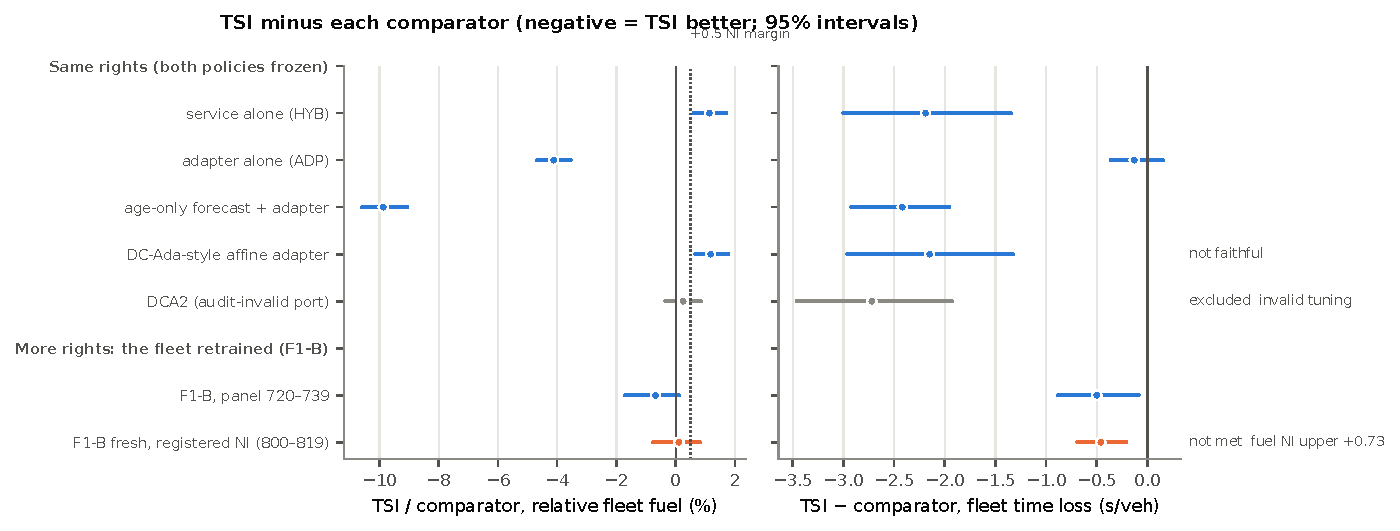
\includegraphics[width=0.9\textwidth]{figs_two_pop/p6_comparators.pdf}
\caption{TSI minus each comparator (negative = TSI better; 95\% intervals). Dotted: the registered $+0.5$ percentage-point
relative-fuel non-inferiority margin. Historical plotted contrasts are not the W8-2 test, which did not establish fuel non-inferiority. The DCA2 row is an archived implementation result, excluded from fair-method claims.}\label{fig:comparators}\end{figure*}

\subsection{M4: Other Networks}\label{sec:m4}
Spider network (own-built, \texttt{netgenerate}): a learned all-green light beats the static programs by 57\,s/veh city time loss (two light seeds, development
traffic, C-76); the rule fleet saves $9.2\%$ fuel against $\sigma^*$ (development traffic, C-77), with agent / human time-loss non-inferiority not established on fresh traffic
(upper $+0.55$ / $+0.52$ against the $+0.5$ margin, C-81);
the four-parameter search fleet (R9) failed its pilot gate against the rule there (fuel $+0.40\%$ $[+0.25,+0.53]$ on development
traffic, C-80); the M2 loss and harm replicate with the rule fleet (C-81); fixed-window commitment is again worse than the
no-SPaT fallback, with a different decomposition (no fleet contribution detected, C-82). The retrained-fleet check was not run there, because its registered condition (F1-A1 confirmed; M4-A7) failed (C-85). The
earlier RESCO cologne8 attempt failed at the light baseline and is kept as a negative (C-35, C-36).
\paragraph{TSI on the second network (C-123, C-124)} The same procedure (the forecaster generalized to two or three greens, the adapter
in front of the multi-green learned light's current / next-green inputs, per-light calibration on new tuning traffic) was tested in two registered
confirmation attempts on fresh spider traffic with the rule fleet; with two light seeds, both are conditional on these two lights. The service alone is strongly harmful there (attempt 1: $+20.7\%$ fuel, $+59.5$\,s/veh agent time, with about one
teleport per run; attempt 2: $+19.8\%$, $+57.8$); adding the adapter reduces that harm (TSI $-$ service: $-58.1$ / $-56.4$\,s/veh agent time), but the full configuration failed both attempts. Attempt 1: fuel $-1.66\%$
$[-1.99,-1.38]$, and both city time loss ($+0.55$, upper $+0.91$) and agent time loss ($+1.33$, upper $+1.94$) fail; $0.025$ teleports per
run (R: 0). Attempt 2, with a wider adapter grid at $\alpha=0.025$: fuel $-0.31\%$ $[-0.81,+0.16]$ (no fuel reduction shown); city $+1.32$,
agent $+1.43$ and human $+1.20$\,s/veh all fail. Spider changes the network, the phase structure, the light learner and the receiver at
once, so the failure is not attributed to any one of them. The reduction of harm is relative to a very harmful service; it is not a
deployable result.
\paragraph{Third and last spider attempt (W6-6)} Registered after attempts 1--2 failed, it published SPaT only where the timing is
determined (a yellow whose next green serves the link) and nothing elsewhere. Every published answer was checked against the realized
phase trace, with 0 mismatches. The per-light choices were $(0,0)$ and $(1,0.5)$. It failed at $\alpha=0.0125$: fuel $+0.70\%$
$[+0.41,+1.03]$, agent time $+0.91$\,s/veh. On this network the determined cells alone give the rule fleet no fuel benefit.

\paragraph{What the spider diagnosis establishes (W8-1)}
The diagnostic suggests hypotheses but does not isolate a cause. Exact timing on approximate open-loop replay yields fuel $-7.39\%$ and $-6.63\%$. Both replay identity checks KH-1 fail, and one agent-time contrast is $+1.34$\,s/veh; this is neither a verified ceiling nor a feasible closed-loop repair.
The reported MAE $21.48$\,s and bias $-15.50$\,s come from 80,004 \emph{debug event-head predictions}, not 80,004 served vehicle queries. The logger records all event heads at queried light-seconds and stops after about 20,000 rows per trace; the four traces end logging at 728--776\,s of a 5,400\,s episode. Grid4's $3.02$\,s MAE uses different served-call sampling. Their ratio is not a valid cross-network error comparison.
With the service, mean greens increase from 18.9 to 28.7\,s, consistent with a changed closed loop. Restricting service to two-green junctions still costs agents time on four TUNE seeds; service at three-green junctions fares better. Location, demand and group size differ, so this does not causally rule out phase structure. A matched sampling scheme with actual query targets and comparable time windows is needed. The earlier diagnosis figure is omitted because its cross-network error bars compare different estimands.

\paragraph{A third network (W8-4)} rand3, a random planar network with 20 two-green signals (Table~\ref{tab:nets}), runs the whole
pipeline with new policies: fleets trained under FT, learned signals trained on rand3, TSI calibrated per signal, confirmation on fresh
rand3 traffic 700--719. It runs last in the queue.
\TODO{W8-4 NET3 results when job 073 lands.}

\subsection{Robustness of the Frozen Design (Wave 9)}\label{sec:robust}
Wave 9 was registered after the limitations were listed and before any of its code ran (Section~\ref{sec:robustdesign}).
\paragraph{Calibration budget, offline (W9-5c)} Re-applying the registered selection rule to subsets of the four TUNE seeds shows that the
exact per-light choice is noisy: with one, two and three seeds it reproduces the four-seed choice on 35\%, 50\% and 62\% of subsets (ten
lights). A single setting is more stable: $(1,0.5)$ is qualified on 10 of 10 lights with four seeds. This motivates the registered test of
one adapter setting for every light, which would remove the adapter grid from deployment.
\paragraph{Channel, sensing, simulator models, one setting, MaxPressure} Fig.~\ref{fig:robust} collects the wave-9 arms against the no-SPaT
fallback on the fresh-policy panel, the one-setting test on the second fresh-policy panel, and the MaxPressure test.
\TODO{W9 results when jobs 072b and 072c land: per-arm verdicts, the calibration-free verdict, the MaxPressure mechanism prediction.}
\begin{figure*}[t]\centering\includegraphics[width=0.92\textwidth]{figs_two_pop/p8_robust.pdf}
\caption{Wave 9 (95\% intervals against the no-SPaT fallback under the same conditions). Rows marked ``pending'' are registered and
queued; the figure is regenerated from the reports by \texttt{scripts/CITY\_fig\_paper.py}.}\label{fig:robust}\end{figure*}

% =====================================================================================================================================
\section{Discussion}\label{sec:discussion}
\subsection{What the Results Establish}
\begin{itemize}\setlength\itemsep{1pt}
\item \textbf{H1 supported.} After the upgrade the frozen fleet's benefit is lost (exactly 0 with the timing withdrawn) and the old program
served as SPaT harms it, on grid4 and on spider.
\item \textbf{H2 supported in the families tried.} No commitment, gate, abstention or predictable split controller met the limits; the
service alone and the adapter alone fail in the saved ablation panels; some reuse the same checkpoints.
\item \textbf{H3 supported, with no single mediator isolated.} Publication lowers the observed halting and lengthens greens; the published
forecast errs more than the shadow forecast; a light-side input change halves this sensitivity; Theorem~\ref{thm:twosided} shows the
pattern holds in the constructed finite model under its stated response and cost definitions, not for arbitrary learned receivers.
\item \textbf{H4 supported on grid4.} TSI met every limit in the registered second attempt ($\alpha=0.025$; chain bound 0.075 by
Theorem~\ref{thm:fwer}), on a third traffic panel, and with five new signals and four new fleets recalibrated from scratch; each half
alone failed in the tested ablation panels. A second fresh-policy panel also passes, but does not establish fuel non-inferiority to retraining. The audited DC-Ada-derived code cannot support a fair published-method comparison.
\item \textbf{H5 partly supported.} Under higher demand, for a rule and a search-fitted fleet and at a 75\% share the frozen design stayed
within the limits; at 25\% the bound sits at the margin. On spider the method failed; its cause remains incompletely isolated. The wave-9 tests are
\TODO{fill when 072b / 072c land}.
\end{itemize}

\subsection{Shortcomings and Limitations}
The list below is what remains after the follow-up experiments; each item states what was done about it.
\begin{itemize}\setlength\itemsep{1pt}
\item \emph{Network generality.} TSI is confirmed on one network family (grids). On spider it failed three registered attempts; the
diagnostics suggest forecast and closed-loop problems but do not isolate a single cause. A third, irregular network
(rand3) is registered and queued.
\item \emph{Simulation only.} No field data. Wave 9 tests the two simulator models most likely to matter (fuel model, car-following model)
\TODO{state the outcome}; a transfer from simulator to site remains untested.
\item \emph{Deployment cost.} Per-signal calibration needs a simulator of the site (8 logged episodes for the forecaster and 44 for the
adapter grid). The offline analysis shows one adapter setting qualified on every light, and its registered test on unseen policies is
queued; the forecaster still needs logs of the deployed signal.
\item \emph{Comparator coverage.} The DC-Ada-derived port has an invalid tuning reference and initialization mismatch; a corrected published-method comparison remains outstanding. Statistical and supervised SPaT predictors appear as service-only arms. CoTV, HONEST-CAV and DHCP were not reproduced. W8-2 does not establish fuel non-inferiority to retraining (upper $+0.728\%$ versus margin $+0.5\%$), despite lower city and agent time losses.
\item \emph{Signal families.} The learned signals are keep-or-switch DQNs on halting counts (and an all-green variant on spider). A
published adaptive signal with all-speed counts (MaxPressure) is tested with a registered mechanism prediction \TODO{outcome}.
\item \emph{Provenance of the first chain.} The rows of the first TSI chain carry no launch-time hash record; their provenance rests on file
times and current hashes (C-128). The fresh-policy replications and later waves record provenance at capture.
\end{itemize}
Evidence is no longer restricted to reused checkpoints: W7-1 and W8-2 add new signals and fleets, recalibrated on grid4. Historical checkpoint reuse and missing launch hashes still apply to the original chain. Neither a faithful published-method comparison nor an isolated cause of second-network failure has been obtained. Corrected provider details are in Appendix~\ref{app:errors}.

\subsection{Open Problems}
\begin{itemize}\setlength\itemsep{1pt}
\item \emph{Forecasts that anticipate their own effect.} One hypothesis for spider is that publication shifts the forecast target. A provider
trained on logs collected \emph{with} the service published, iterated to a fixed point (repeated retraining in the performative sense
\cite{perdomo2020}), is the natural next repair; whether it converges with a learned signal in the loop is open.
\item \emph{A loop-gain measurement.} The small-gain reading predicts that the adapter works by reducing the loop gain; a direct
measurement of that gain, rather than of its consequences, is not available.
\item \emph{Larger formal models.} Theorem~\ref{thm:twosided} has one car and one decision. A model with queues and a stochastic arrival
process that yields a quantitative condition for when the fleet-side half alone suffices would turn the MaxPressure prediction into a
derived statement.
\end{itemize}

% =====================================================================================================================================
\section{Conclusion}\label{sec:conclusion}
Replacing fixed-time signals with learned adaptive signals can improve traffic overall while removing a frozen learned fleet's incremental benefit. Grid4 publication, input-intervention and replay diagnostics support a feedback account involving halting-based observations, without identifying every mediator. The combined forecast and demand-input interface meets the constrained objective where its tested components do not, with confirmation on fresh traffic and two sets of newly trained policies, recalibrated per signal. Neither deployed control policy's weights are updated. Failure on spider, an unresolved published-method comparison and unestablished fuel non-inferiority to retraining remain substantive boundaries. Deployment should evaluate the timing service together with the traffic and signal responses it induces.

\section*{Acknowledgment}
Simulations use SUMO; the formal development uses the Lean~4 theorem prover and the mathlib library.

\begin{thebibliography}{00}\footnotesize
\bibitem{alqithami2026} S.~Alqithami. DC-Ada: Reward-only decentralized sensor adaptation for heterogeneous multi-robot teams. \emph{IEEE Access}, 2026. doi:10.1109/ACCESS.2026.3687163; arXiv:2604.03905.
\bibitem{asadi2011} B.~Asadi, A.~Vahidi. Predictive cruise control: Utilizing upcoming traffic signal information for improving fuel economy and reducing trip time. \emph{IEEE Trans. Control Syst. Technol.} 19(3):707--714, 2011.
\bibitem{ault2021} J.~Ault, G.~Sharon. Reinforcement learning benchmarks for traffic signal control. \emph{NeurIPS Datasets and Benchmarks Track}, 2021.
\bibitem{bansal2019} G.~Bansal, B.~Nushi, E.~Kamar, D.~S.~Weld, W.~S.~Lasecki, E.~Horvitz. Updates in human-AI teams: Understanding and addressing the performance/compatibility tradeoff. \emph{Proc. AAAI}, 2019.
\bibitem{bodenheimer2014} R.~Bodenheimer, A.~Brauer, D.~Eckhoff, R.~German. Enabling GLOSA for adaptive traffic lights. \emph{IEEE Vehicular Networking Conference (VNC)}, 167--174, 2014.
\bibitem{bottom2000} J.~A.~Bottom. \emph{Consistent Anticipatory Route Guidance}. PhD thesis, Massachusetts Institute of Technology, 2000.
\bibitem{dashkovskiy2007} S.~Dashkovskiy, B.~S.~R\"uffer, F.~R.~Wirth. An ISS small gain theorem for general networks. \emph{Math. Control Signals Systems} 19(2):93--122, 2007.
\bibitem{drusvyatskiy2023} D.~Drusvyatskiy, L.~Xiao. Stochastic optimization with decision-dependent distributions. \emph{Math. Oper. Res.} 48(2):954--998, 2023.
\bibitem{eteifa2025} S.~Eteifa, A.~Shafik, H.~Eldardiry, H.~A.~Rakha. Deep learning ensemble approach for predicting expected and confidence levels of signal phase and timing information at actuated traffic signals. \emph{Sensors} 25:1664, 2025. doi:10.3390/s25061664.
\bibitem{genser2024} A.~Genser, M.~A.~Makridis, K.~Yang, L.~Amb\"uhl, M.~Menendez, A.~Kouvelas. Time-to-green predictions for fully-actuated signal control systems with supervised learning. \emph{IEEE Trans. Intell. Transp. Syst.}, doi:10.1109/TITS.2023.3348634; arXiv:2208.11344.
\bibitem{gu2025} H.~Gu, Y.~Zhang, C.~Wang, R.~Jiang, Z.~Qiao, P.~Fan, D.~Jia. A hierarchical deep reinforcement learning framework for traffic signal control with predictable cycle planning. arXiv:2509.03118, 2025.
\bibitem{guo2023} J.~Guo, L.~Cheng, S.~Wang. CoTV: Cooperative control for traffic light signals and connected autonomous vehicles using deep reinforcement learning. \emph{IEEE Trans. Intell. Transp. Syst.} 24(10), 2023. arXiv:2201.13143.
\bibitem{hu2020} H.~Hu, A.~Lerer, A.~Peysakhovich, J.~Foerster. ``Other-play'' for zero-shot coordination. \emph{Proc. ICML}, PMLR 119:4399--4410, 2020.
\bibitem{huang2026} Z.~Huang, Y.~Liu, C.~Liang, G.~Zheng. Planning under observation mismatch for traffic signal control via adaptive modular world models. \emph{ICAPS}, 2026. arXiv:2501.02548.
\bibitem{jiang1994} Z.-P.~Jiang, A.~R.~Teel, L.~Praly. Small-gain theorem for ISS systems and applications. \emph{Math. Control Signals Systems} 7(2):95--120, 1994.
\bibitem{katsaros2011} K.~Katsaros, R.~Kernchen, M.~Dianati, D.~Rieck. Performance study of a Green Light Optimized Speed Advisory (GLOSA) application using an integrated cooperative ITS simulation platform. \emph{IWCMC}, 918--923, 2011. doi:10.1109/IWCMC.2011.5982524.
\bibitem{lopez2018} P.~A.~Lopez, M.~Behrisch, L.~Bieker-Walz, J.~Erdmann, Y.-P.~Fl\"otter\"od, R.~Hilbrich, L.~L\"ucken, J.~Rummel, P.~Wagner, E.~Wie{\ss}ner. Microscopic traffic simulation using SUMO. \emph{IEEE ITSC}, 2018. doi:10.1109/ITSC.2018.8569938.
\bibitem{narang2023} A.~Narang, E.~Faulkner, D.~Drusvyatskiy, M.~Fazel, L.~J.~Ratliff. Multiplayer performative prediction: Learning in decision-dependent games. \emph{J. Mach. Learn. Res.} 24(202):1--56, 2023.
\bibitem{perdomo2020} J.~Perdomo, T.~Zrnic, C.~Mendler-D\"unner, M.~Hardt. Performative prediction. \emph{Proc. ICML}, PMLR 119:7599--7609, 2020.
\bibitem{stone2010} P.~Stone, G.~A.~Kaminka, S.~Kraus, J.~S.~Rosenschein. Ad hoc autonomous agent teams: Collaboration without pre-coordination. \emph{Proc. AAAI}, 2010.
\bibitem{varaiya2013} P.~Varaiya. Max pressure control of a network of signalized intersections. \emph{Transportation Research Part C}, 2013.
\bibitem{wei2018} H.~Wei, G.~Zheng, H.~Yao, Z.~Li. IntelliLight: A reinforcement learning approach for intelligent traffic light control. \emph{Proc. KDD}, 2018.
\bibitem{wei2019} H.~Wei, C.~Chen, G.~Zheng, K.~Wu, V.~Gayah, K.~Xu, Z.~Li. PressLight: Learning max pressure control to coordinate traffic signals in arterial network. \emph{Proc. KDD}, 2019.
\bibitem{zhang2026} Z.~Zhang, C.~Wan, P.~Hao, K.~Boriboonsomsin, M.~J.~Barth, Y.~Liu, S.~Ucar, G.~Wu. HONEST-CAV: Hierarchical optimization of network signals and trajectories for connected and automated vehicles with multi-agent reinforcement learning. arXiv:2602.18740, 2026.
\bibitem{shen2020} Y.~Shen, Y.~Xiong, W.~Xia, S.~Soatto. Towards backward-compatible representation learning. \emph{Proc. CVPR}, 2020.
\bibitem{yan2021} S.~Yan, Y.~Xiong, K.~Kundu, S.~Yang, S.~Deng, M.~Wang, W.~Xia, S.~Soatto. Positive-congruent training: Towards regression-free model updates. \emph{Proc. CVPR}, 2021.
\bibitem{reitblatt2012} M.~Reitblatt, N.~Foster, J.~Rexford, C.~Schlesinger, D.~Walker. Abstractions for network update. \emph{Proc. ACM SIGCOMM}, 2012.
\bibitem{nguyen2026legacy} V.~P.~A.~Nguyen. Upgrading communication without retraining every agent: Legacy-view emulation for mixed-version MARL. Manuscript in preparation, 2026.
\bibitem{mahler2014} G.~Mahler, A.~Vahidi. An optimal velocity-planning scheme for vehicle energy efficiency through probabilistic prediction of traffic-signal timing. \emph{IEEE Trans. Intell. Transp. Syst.} 15(6):2516--2523, 2014.
\bibitem{vanhasselt2016} H.~van Hasselt, A.~Guez, D.~Silver. Deep reinforcement learning with double Q-learning. \emph{Proc. AAAI}, 2016.
\bibitem{schulman2017} J.~Schulman, F.~Wolski, P.~Dhariwal, A.~Radford, O.~Klimov. Proximal policy optimization algorithms. arXiv:1707.06347, 2017.
\bibitem{krauss1998} S.~Krau{\ss}. \emph{Microscopic Modeling of Traffic Flow: Investigation of Collision Free Vehicle Dynamics}. PhD thesis, University of Cologne, 1998.
\bibitem{treiber2000} M.~Treiber, A.~Hennecke, D.~Helbing. Congested traffic states in empirical observations and microscopic simulations. \emph{Phys. Rev. E} 62(2):1805--1824, 2000.
\bibitem{krajzewicz2015} D.~Krajzewicz, M.~Behrisch, P.~Wagner, R.~Luz, M.~Krumnow. Second generation of pollutant emission models for SUMO. In \emph{Modeling Mobility with Open Data}, Springer, 2015, pp.~203--221.
\bibitem{owen2007} A.~B.~Owen. The pigeonhole bootstrap. \emph{Ann. Appl. Stat.} 1(2):386--411, 2007.
\bibitem{efron1993} B.~Efron, R.~J.~Tibshirani. \emph{An Introduction to the Bootstrap}. Chapman \& Hall, 1993.
\bibitem{moura2021} L.~de~Moura, S.~Ullrich. The Lean 4 theorem prover and programming language. \emph{Proc. CADE}, LNCS 12699, 2021.
\bibitem{mathlib2020} The mathlib Community. The Lean mathematical library. \emph{Proc. CPP}, 2020, pp.~367--381.
\end{thebibliography}

\appendices
\section{Reproducibility}\label{app:repro}
Registered endpoints come from registered report scripts over saved per-episode rows; every other number comes from the same saved rows
through the analysis named in its ledger row, and the post-hoc ones are labelled (C-55, C-101, C-117, C-125, C-126, C-128).
Provenance gap: the TSI, TSI-2, SHIFT, GEN and spider protocols have no launch-time hash record, and the TSI / HYB rows do not carry the
forecaster, fleet or table hashes (the evaluator's metadata is not written when it is imported; C-128). Every recorded component hash equals
the current source, and every module and input on these paths predates its first use (file times); the freeze record of C-128 lists them. Main files (repository paths):
\begin{itemize}\setlength\itemsep{0pt}
\item protocols: \path{research/city_sim/PROTOCOL_CITY_TSI2_20261005.md} (method and confirmation) and the TSI, SHIFT, GEN, PERF and
SPIDER\_TSI protocols of the same date in the same directory;
\item evaluators: \path{scripts/CITY_eval_n4.py} (grid4 service and \path{--light-obs q:A:B}), run through
\path{scripts/CITY_f1a1_run.py} (loads the light checkpoints t4--t8) and, for fleet shares, \path{scripts/CITY_rho_run.py}; \path{scripts/CITY_m4s_tsi_eval.py} (spider);
\item forecasters: \path{scripts/CITY_n2_fit.py}, \path{scripts/CITY_n2k.py}; calibration: \path{scripts/CITY_tsi2_tune.py};
\item reports: \path{scripts/CITY_tsi2_report.py}, \path{CITY_shift_report.py}, \path{CITY_gen_report.py}, \path{CITY_perf_report.py},
\path{CITY_sptsi_report.py}; figures: \path{scripts/CITY_fig_tsi.py}.
\item wave 6: \path{research/city_sim/PROTOCOL_CITY_WAVE6_20261005.md} (with its pre-run amendment); \path{scripts/CITY_w6_dca_tune.py},
\path{CITY_m4s_tsi3_eval.py}, \path{CITY_w6_m2l.py}, \path{CITY_fleet_train_h45.py}, \path{CITY_lcd.py}, \path{CITY_eval_n9.py}; reports
\path{CITY_w6_report.py} (job 051) and \path{CITY_w6_report_v2.py}; freeze record \path{research/city_sim/FREEZE_RECORD_TSI_20261005.md}.
\end{itemize}
Determinism: \path{PYTHONHASHSEED=0}, \path{OMP_NUM_THREADS=1}. Parity checks KN2 / KT-1 / KS-1 compare offline and online features and
predictions (0 mismatches).

{\sloppy\noindent Later waves: \path{research/city_sim/PROTOCOL_CITY_WAVE7_20261005.md}, \path{PROTOCOL_CITY_WAVE8_20261005.md} and
\path{PROTOCOL_CITY_WAVE9_20261005.md}; runners \path{scripts/CITY_w7_run.py}, \path{CITY_w8_run.py}, \path{CITY_w9_run.py} (run-time
perturbations; no evaluator edited); reports \path{CITY_w7_report.py}, \path{CITY_w8_report.py}, \path{CITY_w8_spdiag.py},
\path{CITY_w9_report.py}, \path{CITY_w9_calbudget.py}; figures \path{scripts/CITY_fig_paper.py}. Lean modules (\path{work/p13_conjectures/}):
\path{LeanCityConditionalShiftV1.lean}, \path{LeanCityReceiverContractV1.lean}, \path{LeanCityTwoSidedV1.lean}.\par}


\section{History of the M1 and M2 Recipes}\label{app:history}
\paragraph{Earlier fleet recipes (C-21 \dots C-37)} No earlier recipe was confirmed (C-21 \dots C-31, corrected C-37); one development checkpoint (R5h\_t0)
passed on fresh traffic; the non-learned $\sigma$-family is a strong baseline ($\sigma=0.3$: $-2.5$ s/veh, $-2.2\%$ fuel).
\paragraph{Fleet diagnostics (C-39 \dots C-43)} D1: the ported phase reward (B) prefers physically better behaviour for large
differences but does not encode the time-loss constraints (it ranks an infeasible fuel-for-time policy far above always-SUMO); PPO from
scratch did not reach always-SUMO even on its training traffic. D2: a hand-written in-class controller (GLOSA target, no release) gives
$-6.7\%$ fuel at equal agent time but harms human cars; a behaviour clone of the heuristic GLOSA trades fuel for time in closed loop.
An evaluation bug (exit release missing in deterministic evaluation) was found by an identity check and fixed (C-41).
A residual on the in-class controller with a crawl-proof group cost (v9) failed its pilot gate; its confirmation was not evaluated (C-47).
Derivative-free policy search over a three-parameter GLOSA family on the deployment objective (fuel with time-loss penalties) returned
the untuned heuristic itself for the pilot search seed; the heuristic fails the $\sigma^*$ comparison on agent time loss (+1.8\,s/veh,
SELECT) and the human-time-loss margin on the width of its 5-seed bound (C-43).
\paragraph{Earlier compatibility probes (C-14 \dots C-34)} Weak learned fleets regressed under light upgrades and a car-side reaction repair
helped (C-14, C-16); non-learned fleet upgrades ($\sigma$, ACC) were not harmed by three learned-light families (C-30, C-32 \dots C-34).

\section{Candidates That Failed, and Errors Found and Fixed}\label{app:errors}
\paragraph{Failed candidates (all reported in the ledger)} M3-E reward-shaped lights (DEV); fixed-window, ETA and receiver-triggered
commitments (WC5, RPC confirmed worse than the fallback, C-86; RPC $2\times2$ diagnostic C-95); per-decision commitment selection (no
selection rule better than a random option out of sample, every interval includes 0; C-96, C-98); tail-support abstention (C-97);
confidence / horizon gates and gate + adapter (C-104, C-105); a CEM-tuned
committed-duration controller (C-116); TSI variants (direct-only hybrid, no SPaT on permissive lefts; C-119); TSI first confirmation
(C-114); spider attempts 1 and 2 (C-123, C-124).
\paragraph{Errors found and fixed} Found after results that used them, and disclosed with those results: the SPaT timing convention
($+1$\,s, C-71; M2b used the earlier provider) and a yellow branch left 1\,s early by the first correction (C-84, found by an audit;
corrected in the provider c2 for all later runs). Found by self-checks or job failures before the verdict they affected: an xargs job-merging bug (C-92); an exactness error in the committed-duration controller's SPaT (two fixes, KN8-1, C-112);
missing output directories (C-112); a tuple error in the spider provider, caught by KS-2 (C-123 Amendment A1). One provider file was edited
while a job imported it, with no change to the registered code paths (C-103).
Reporting errors corrected in the text: ``exact in yellow'' had been claimed from the 0.1-quantile table (C-113); the spider attempt-2
report header prints attempt 1's traffic range (C-124); the scope report's limits line skipped teleports (C-126); the demand-shift report tested neither teleports nor unfinished trips (both 0
in its 600 runs, C-128); the spider attempt-2 amendment states it was registered before attempt 1's result was read, which the file
times cannot verify (attempt 1's per-seed log lines were printed before the attempt-2 job list was written; C-128).
\section{Validation and Pitfalls (QA)}\label{app:qa}
Checks that failed during development, each of which changed what was reported:
\begin{itemize}\setlength\itemsep{1pt}
\item \emph{Impossible rewards} (C-22). Training logs of one fleet arm showed positive mean rewards for a non-negative cost; the reward was
read from the wrong field, and the arm was declared invalid.
\item \emph{An action class that did not contain the base driver} (C-25, C-27). Under a persistent \texttt{setSpeed}, a zero residual means
``never accelerate'': a car stopped at red stays stopped. Constant release reproduced SUMO's own driving bit for bit, while the zero
residual jammed the network; residual fleets were redesigned on the rule with release.
\item \emph{A fleet worse in every cell} (C-17). Early learned fleets were worse than the same vehicles driven by SUMO in all 65 runs; this
led to the $\sigma$-family baseline and to M1 as a precondition.
\item \emph{A timing convention off by one second} (C-38). The first trace check of the SPaT feature found every prediction 1\,s late
(39\,522 of 39\,522), showing that the check can fail; the convention was fixed and declared.
\item \emph{Horizon semantics} (C-133). A Lagrangian reference measured to 5\,400\,s was subtracted from training episodes of 3\,600\,s;
corrected before the run.
\item \emph{Determinism} (C-27). Python's set-order hashing moved time losses by up to 1.45\,s/veh between identical runs;
\path{PYTHONHASHSEED=0} is mandatory, and \path{OMP_NUM_THREADS=1} is bit-identical.
\item \emph{Over-strong wording} (C-37). ``No learned fleet can be beneficial'' was corrected to ``no recipe was confirmed in the settings
tried''; a failed test is not reported as its converse.
\end{itemize}


\end{document}
